\documentclass[pdflatex,onecolumn,sn-mathphys-num]{sn-jnl}
% LSCBO scheduler: task-reassignment local search with Levy-assisted CBO for Cloud Task Scheduling
% Cloud meta-heuristic format: scheduling model + algorithm improvement + CEC2017 + CloudSim

\usepackage{graphicx}
\usepackage{multirow}
\usepackage{amsmath,amssymb,amsfonts}
\usepackage{amsthm}
\usepackage[title]{appendix}
\usepackage{xcolor}
\usepackage{textcomp}
\usepackage{manyfoot}
\usepackage{booktabs}
\usepackage{algorithm}
\usepackage{algorithmicx}
\usepackage{algpseudocode}
\usepackage{listings}
\usepackage{microtype}
\usepackage{float}
\usepackage{placeins}
\emergencystretch=3em
\hfuzz=2pt
\vfuzz=2pt
\hbadness=10000
\vbadness=10000
\raggedbottom
\hypersetup{hypertexnames=false}

\begin{document}

\title[LSCBO Scheduler]{LSCBO Scheduler: Task-Reassignment Local Search for CBO-Based Multi-Cost Cloud Task Scheduling}

\author*[1]{\fnm{First} \sur{Author}}\email{first.author@example.com}

\affil*[1]{\orgdiv{Department or School}, \orgname{University Name}, \orgaddress{\city{City}, \country{China}}}

\abstract{
Effective task scheduling is essential for reducing resource waste, operating cost, and service delay in cloud computing environments. The complexity of cloud task scheduling requires algorithms that can search globally while also exploiting the structure of task-to-VM assignment. This paper proposes LSCBO (L\'{e}vy-assisted Local-Search Coyote-Badger Optimization), a cloud-oriented scheduler that augments the Coyote-Badger Optimization (CBO) framework by combining task-reassignment local search with L\'{e}vy-assisted stochastic exploration. The task-reassignment operator redistributes tasks from overloaded to underloaded virtual machines before execution, while the L\'{e}vy perturbation supplies auxiliary global-search diversity.

The proposed scheduler is evaluated in two experimental series following the standard validation pattern for cloud meta-heuristic scheduling studies. First, LSCBO is tested on 29 CEC2017 benchmark functions to verify its general optimization capability. In this setting, LSCBO obtains the lowest Friedman average rank (1.86) within the seven-optimizer comparison, with statistically significant wins over CBO, PSO, SA, and GWO ($p < 0.001$), and statistical parity with DE ($p = 0.059$) and GTO ($p = 0.481$). Second, LSCBO is applied to multi-cost cloud task scheduling in a CloudSim Plus scheduling pipeline---with all 12,780 formal rows executed through full CloudSim Plus simulation---and compared with eight population-based meta-heuristic schedulers under identical task, VM, seed, population-size, and iteration settings; the additional local-search evaluations used by LSCBO are explicitly counted and reported rather than absorbed into a nominally identical evaluation budget.

In the formal 12,780-row cloud scheduling experiment, LSCBO obtains the lowest average objective rank of 1.087 within the nine-scheduler meta-heuristic comparison. Relative to the standardized CBO baseline, LSCBO improves makespan by 9.6\%--30.1\%, energy by 7.3\%--24.1\%, load imbalance by 8.8\%--24.7\%, and the overall scalarized objective by 7.4\%--22.6\% across the five task scales. Component analysis shows that task-reassignment local search is the dominant performance driver, while L\'{e}vy perturbation supplies a smaller and less stable auxiliary contribution. Further robustness tests across scalarization weights and VM heterogeneity settings show that LSCBO maintains the best average objective rank within the evaluated meta-heuristic scheduler family. These results support the narrower claim that combining a CBO search framework with scheduling-specific task reassignment is an effective design pattern within the evaluated family of cloud meta-heuristic schedulers.
}

\keywords{Cloud Task Scheduling, Coyote-Badger Optimizer, L\'{e}vy Flight, Task-Reassignment Local Search, CEC2017 Benchmarks, Meta-Heuristic Scheduling}

\maketitle

\section{Introduction}\label{sec1}

\subsection{Background and Motivation}
Cloud computing platforms must continuously assign thousands of heterogeneous tasks to heterogeneous Virtual Machines (VMs) while optimizing multiple objectives including makespan, energy consumption, monetary cost, and load balance. With the rapid growth of Internet of Things (IoT), big data analytics, and artificial intelligence workloads, the resulting Cloud Task Scheduling Problem (CTSP) has become increasingly large-scale and complex, rendering exact optimization methods such as branch-and-bound or dynamic programming impractical for real-time scheduling decisions~\cite{Braun2001,Etminani2007}.

Population-based meta-heuristics have emerged as a practical alternative for solving the CTSP. These algorithms can provide high-quality approximate solutions across diverse problem domains without requiring gradient information or problem-specific exact formulations. Recent years have witnessed a surge of novel nature-inspired optimizers, including Harris Hawks Optimization (HHO)~\cite{Heidari2019}, Whale Optimization Algorithm (WOA)~\cite{Mirjalili2016}, Grey Wolf Optimizer (GWO)~\cite{Mirjalili2014}, Dung Beetle Optimizer (DBO)~\cite{Xue2022}, Artificial Gorilla Troops Optimizer (GTO)~\cite{Abdollahzadeh2021}, and Coyote-Badger Optimization (CBO)~\cite{Khatab2025}. Many of these algorithms employ phase-based search structures that decompose the optimization process into distinct behavioral stages, and several scheduling-oriented variants have incorporated additional operators such as L\'{e}vy flight, chaotic mapping, or problem-specific heuristics to improve convergence~\cite{Chintale2024,Sabipour2025,Zhu2025,Xie2024}.

Despite these advances, three key challenges remain: (1) maintaining an effective balance between global exploration and local exploitation in high-dimensional scheduling landscapes, (2) ensuring rigorous and transparent statistical evaluation protocols for algorithm comparisons, and (3) providing systematic component-level analysis that identifies which algorithmic mechanisms genuinely contribute to performance.

\subsection{Proposed Scheduler: LSCBO}
To address these challenges, we propose LSCBO (L\'{e}vy-assisted Local-Search CBO), a population-based meta-heuristic scheduler that extends the CBO framework with two enhancements: (1) a greedy task-reassignment local search that exploits the scheduling problem structure by redistributing tasks from overloaded to underloaded VMs before execution, and (2) L\'{e}vy-flight exploration that replaces the original deterministic tanh-based searching operator and provides stochastic perturbation for global search. The name encodes these two additions to CBO: the ``L'' denotes the L\'{e}vy-flight search and the ``S'' the task-reassignment local search. We emphasize at the outset that, although the L\'{e}vy component is retained in the algorithm name, the empirical analysis in this paper (perturbation-mechanism comparison in Section~\ref{sec:perturbation} and component ablation in Section~\ref{sec:phase_ablation}) identifies task-reassignment local search as the dominant performance driver; L\'{e}vy flight is kept as an auxiliary search-diversity mechanism and is \emph{not} claimed as an independent source of performance gain.

CBO is selected as the base framework for its modular three-phase architecture (searching, encircling, attacking), which enables controlled component modification without disrupting other phases. LSCBO preserves the encircling and attacking phases of CBO unchanged while enhancing the searching phase with stochastic exploration and augmenting the overall optimization process with problem-specific exploitation. The resulting scheduler follows the common cloud meta-heuristic design pattern: a general optimizer provides global search, while a scheduling-specific operator improves feasible task-to-VM assignments. The experiments below therefore interpret L\'{e}vy flight as an auxiliary search perturbation and task reassignment as the principal cloud-scheduling mechanism.

\subsection{Contributions}
The main contributions of this work are:

\begin{itemize}
    \item \textbf{A cloud-oriented CBO scheduler:} We propose LSCBO, a CBO-based task scheduler that combines task-reassignment local search with L\'{e}vy-flight stochastic exploration for multi-cost cloud task scheduling.
    
    \item \textbf{Comprehensive two-series experimental validation:} We evaluate LSCBO through two complementary experimental campaigns: (i) 29 CEC2017 global optimization functions (F1, F3--F30) to validate its general optimization capability, and (ii) formal multi-cost scheduling experiments against population-based meta-heuristic schedulers across 5 task scales, 5 weight configurations, 3 VM heterogeneity regimes, perturbation mechanism comparisons, and component-level ablation.
    
    \item \textbf{Task-reassignment local search for cloud scheduling:} A greedy local-search operator that exploits the scheduling structure by reassigning tasks from the most-loaded to the least-loaded VM is shown to be the dominant performance driver in the cloud scheduling experiments; L\'{e}vy perturbation is treated as a secondary global-search aid.
    
    \item \textbf{Systematic component ablation and evolution-path analysis:} A five-stage evolution-path experiment traces the development from CBO to LSCBO, while component ablation separates the influence of local search, L\'{e}vy perturbation, and preserved CBO phases.
    
    \item \textbf{Robustness validation across optimization preferences and VM configurations:} LSCBO's performance within the meta-heuristic scheduler family is empirically validated across five scalarization weight configurations and three VM heterogeneity regimes.
\end{itemize}

\section{Related Work}\label{sec2}

\subsection{Multi-Cost Cloud Task Scheduling Models}
Cloud task scheduling has been studied through deterministic dispatching rules, population-based meta-heuristics, learning-based schedulers, and Pareto-front multi-objective methods. Classical rules such as Min-Min, Max-Min, and FCFS remain useful background methods because they are simple and fast~\cite{Braun2001,Etminani2007}. However, their fixed decision logic is often insufficient when heterogeneous VMs, large task sets, and several cost criteria must be considered together.

The central modeling issue is that a schedule should not be judged only by completion time. Energy consumption, monetary cost, and load imbalance also influence whether a task-to-VM assignment is useful in a cloud platform. Pareto-front approaches such as NSGA-II~\cite{Deb2002} and MOEA/D~\cite{Zhang2007} directly approximate trade-off surfaces, whereas many cloud meta-heuristic schedulers use a normalized scalar objective so that several criteria can be optimized by one search process. The present paper follows the latter protocol and therefore evaluates LSCBO under a scalarized multi-cost model, while acknowledging that Pareto-front scheduling is a separate experimental setting.

\subsection{Meta-Heuristic Schedulers for Cloud Task Assignment}
Population-based meta-heuristics are widely used for cloud task scheduling because they can search large combinatorial spaces without requiring gradient information. Classical foundations include Particle Swarm Optimization (PSO)~\cite{Kennedy1995} and Genetic Algorithms (GA)~\cite{Goldberg1989}; in discrete scheduling, continuous positions are converted into task orders or assignment decisions through rules such as Smallest Position Value (SPV)~\cite{Tasgetiren2007}. More recent optimizers provide a diverse set of search templates, including Harris Hawks Optimization (HHO)~\cite{Heidari2019}, Whale Optimization Algorithm (WOA)~\cite{Mirjalili2016}, Grey Wolf Optimizer (GWO)~\cite{Mirjalili2014}, Dung Beetle Optimizer (DBO)~\cite{Xue2022}, Kepler Optimization Algorithm (KOA)~\cite{AbdelBasset2023,Qian2025}, Arithmetic Optimization Algorithm (AOA)~\cite{Abualigah2021}, Artificial Gorilla Troops Optimizer (GTO)~\cite{Abdollahzadeh2021}, Snake Optimizer (SO)~\cite{Hashim2022}, Snow Ablation Optimizer (SAO)~\cite{Deng2023}, Pelican Optimization Algorithm (POA)~\cite{Trojovska2022}, Marine Predators Algorithm (MPA)~\cite{Faramarzi2020}, Reptile Search Algorithm (RSA)~\cite{Abualigah2022}, and Artificial Rabbits Optimization (ARO)~\cite{Wang2022}.

When these optimizers are adapted to cloud task scheduling, the main research problem is no longer only how to improve a generic search equation. The scheduler must also encode a continuous-to-discrete mapping, preserve feasible assignments, and evaluate candidates under the same cost model. Recent cloud-oriented variants reflect this pattern: enhanced DBO scheduling~\cite{Xie2024}, E-AVOA-TS~\cite{Ghafari2023}, GTO-based fault-tolerant scheduling~\cite{Rengaraj2023}, ERTH with elite strategies and chaotic mapping~\cite{Ferahtia2023,Qin2024}, CEEO for IoT-generated cloud tasks~\cite{EbrahimiMood2025}, and DECSO for multi-objective cloud scheduling~\cite{Gunduz2025}. These works are used here as methodological context rather than as direct experimental baselines.

\subsection{Problem-Specific Hybridization and Local Search}
Hybridization is common in cloud meta-heuristic scheduling, but not every added operator contributes equally. L\'{e}vy-enhanced Osprey Optimization~\cite{Dehghani2023,Chintale2024}, chaotic RIME with generalized quadratic interpolation and L\'{e}vy flight~\cite{Sabipour2025}, and hybrid SAO-RIME scheduling~\cite{Zhu2025} show that stochastic perturbations can improve search diversity. The Mantegna scheme provides a standard way to generate stable L\'{e}vy-distributed steps~\cite{Mantegna1994}, and L\'{e}vy flight was introduced prominently into Cuckoo Search by Yang and Deb~\cite{Yang2009}.

For cloud scheduling, however, diversity alone is not enough. The reviewed literature suggests that the strongest gains occur when a meta-heuristic is coupled with a mechanism that understands the scheduling structure. This is the role of task-reassignment local search in LSCBO: after a candidate assignment has been decoded, the scheduler tests whether moving tasks from the most-loaded VM toward the least-loaded VM improves the scalarized objective. This follows the memetic principle of coupling a general optimizer with a problem-specific local improvement operator~\cite{Moscato1989}.

\subsection{Positioning and Comparison Boundary of LSCBO}
The Coyote-Badger Optimization (CBO) framework is inspired by documented coyote-badger interactions~\cite{Kiliaan1991} and formalizes the behavior as a three-phase population search process~\cite{Khatab2025}. For the present work, the biological analogy is not treated as evidence of performance. We are aware of the ongoing methodological debate in the optimization community regarding the proliferation of metaphor-based metaheuristics, and we therefore deliberately ground our design choices in CBO's modular phase structure rather than in its biological narrative. CBO is selected because its searching, encircling, and attacking phases form a modular structure that can be modified and ablated without redesigning the entire optimizer; the component-ablation experiment in Section~\ref{sec:phase_ablation} exploits exactly this modularity to attribute performance to specific mechanisms rather than to the metaphor.

LSCBO is therefore positioned as a CBO-based scheduler with two controlled additions: L\'{e}vy-assisted stochastic exploration and task-reassignment local search. Its direct comparison focuses on population-based meta-heuristic schedulers under identical task, VM, seed, population-size, and iteration settings. Restricting the experimental comparison to other population-based meta-heuristic schedulers follows the established protocol of recent cloud meta-heuristic scheduling studies such as enhanced DBO scheduling~\cite{Xie2024}, E-AVOA-TS~\cite{Ghafari2023}, ERTH~\cite{Ferahtia2023,Qin2024}, and DECSO~\cite{Gunduz2025}, which likewise benchmark against the meta-heuristic family rather than against classical dispatching rules. Deterministic dispatching rules such as Min-Min and Max-Min, DRL schedulers such as DeepRM~\cite{Mao2016} and Decima~\cite{Mao2019}, exact methods, and Pareto-front algorithms remain important adjacent paradigms, but they require different protocols and are therefore treated as methodological context rather than as direct experimental baselines, and are not used as the basis for a universal state-of-the-art claim.

\section{Research Methodology}\label{sec3}

\subsection{Multi-Cost Cloud Task Scheduling Model}\label{sec4}

\subsubsection{System Model}
The cloud datacenter provides $M$ heterogeneous Virtual Machines $V = \{VM_1, \ldots, VM_M\}$ processing $N$ independent tasks $T = \{T_1, \ldots, T_N\}$. The computational capacity is defined by $MIPS_j$ for $VM_j$ and $MI_i$ size for $T_i$. The Expected Time to Compute ($ETC$) is:
\begin{equation}
ETC_{i,j} = \frac{MI_i}{MIPS_j}
\end{equation}
All $N$ tasks are assumed to be known a priori (offline batch scheduling), which is standard in the meta-heuristic scheduling literature~\cite{Braun2001} and appropriate for scenarios such as scientific workflow execution and periodic batch processing. The main notation used throughout this section is summarized in Table~\ref{tab:notation}, and the overall multi-cost scheduling model is illustrated in Fig.~\ref{fig:scheduling_model}.

\begin{figure}[htbp]
\centering
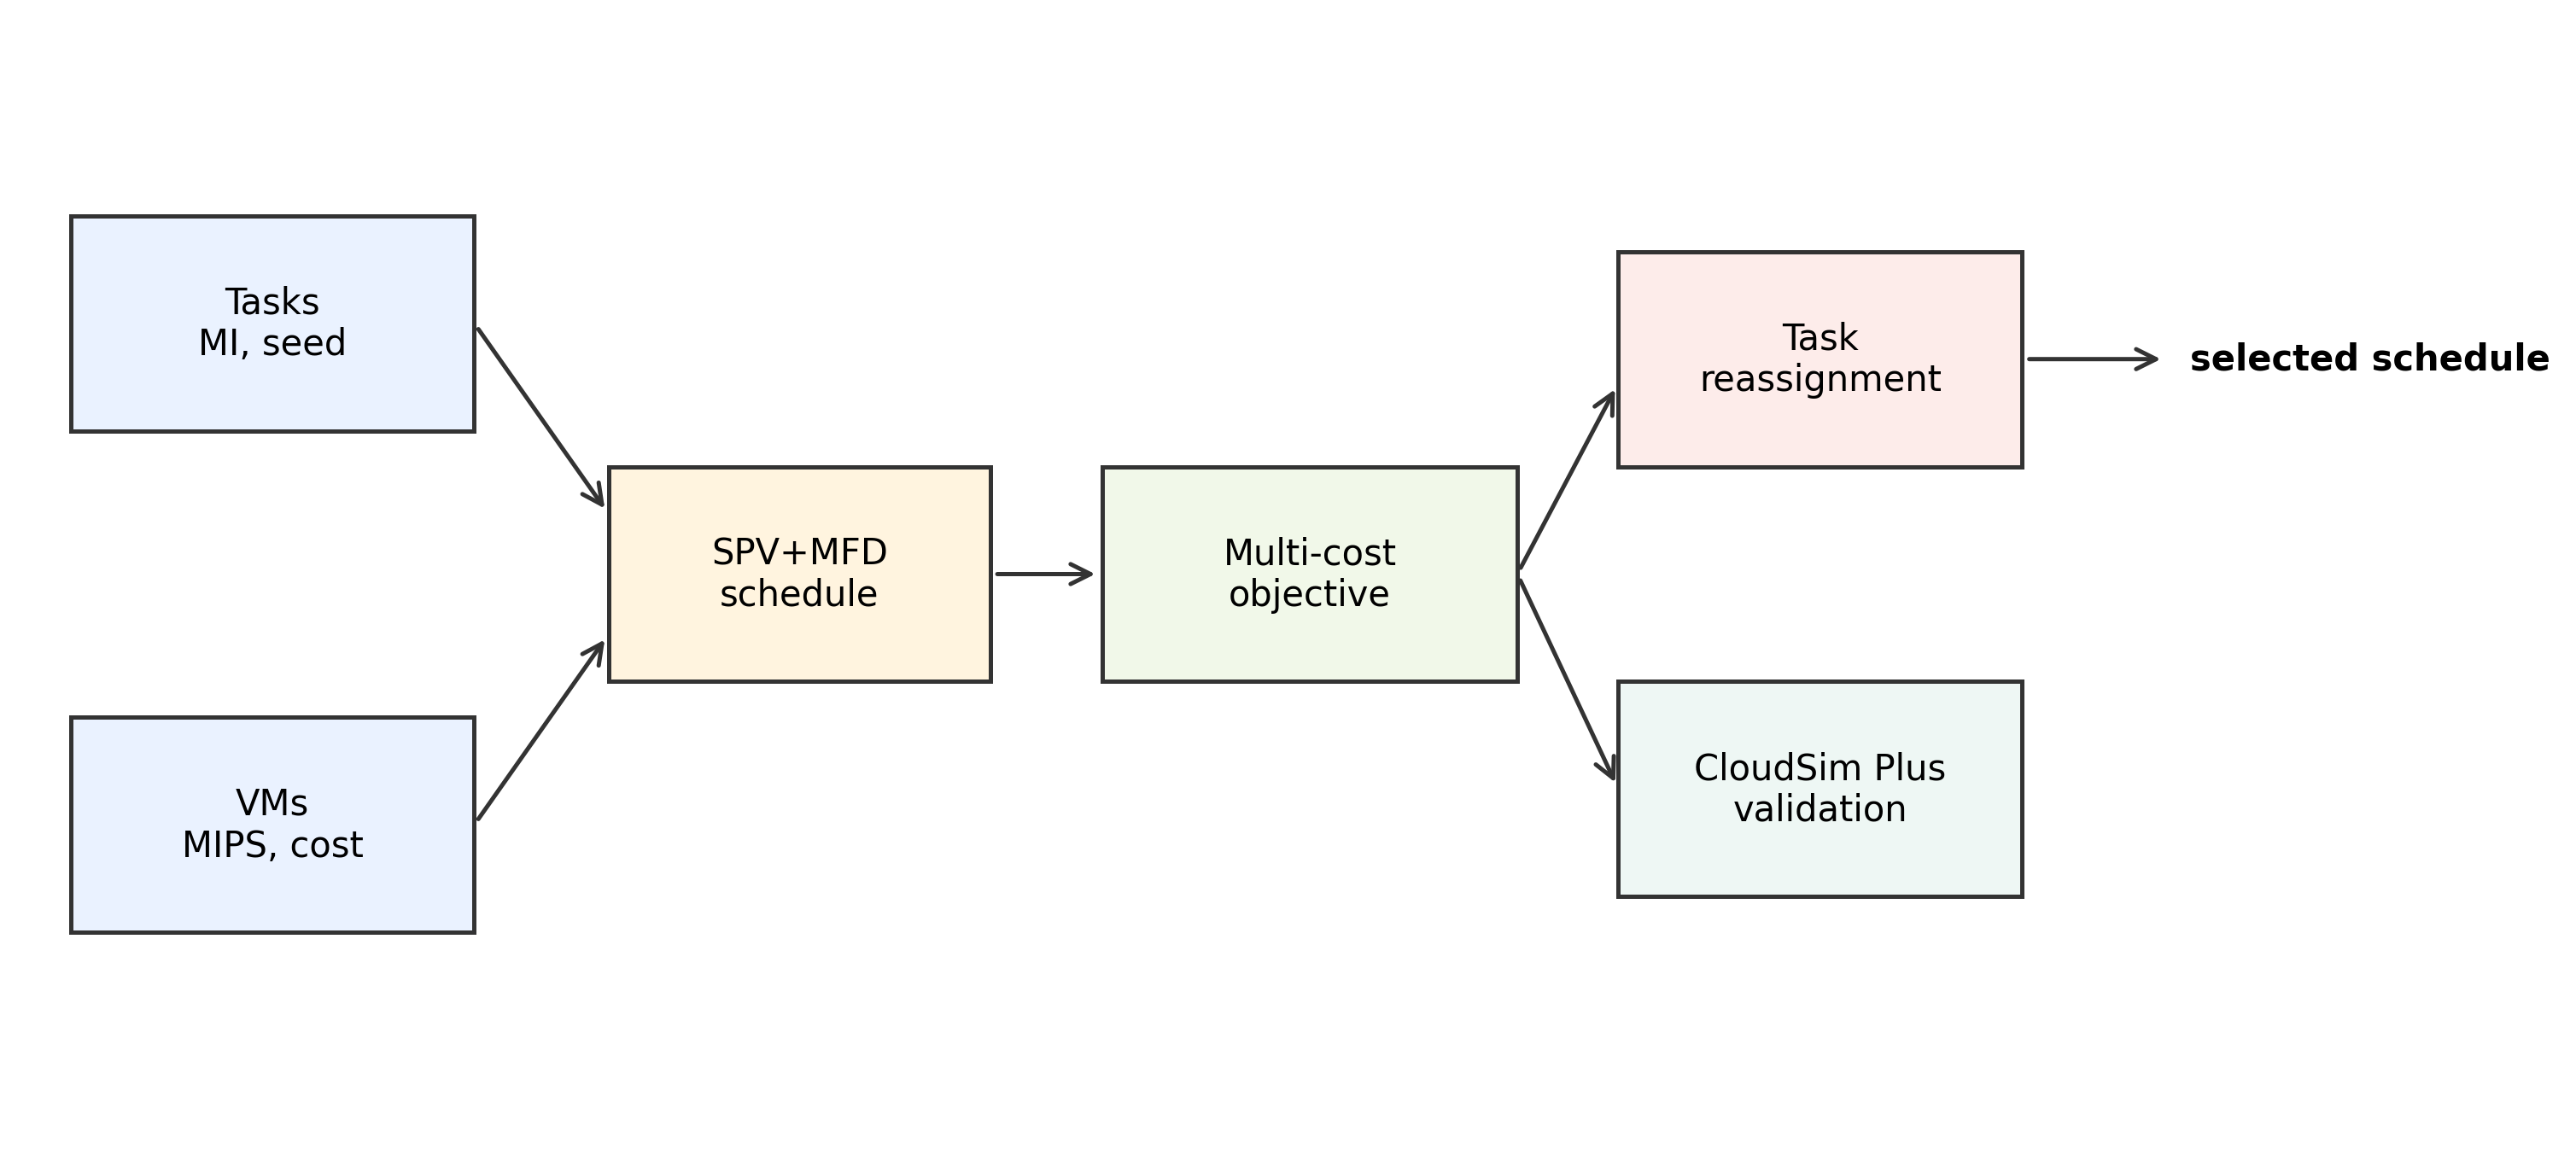
\includegraphics[width=0.92\textwidth]{figures/fig_lscbo_scheduling_model.png}
\caption{Multi-cost cloud task scheduling model used by LSCBO. A continuous population search is decoded into feasible task-to-VM assignments, evaluated by makespan, energy, execution cost, and load-balance criteria, and then improved by task-reassignment local search before the selected schedule is evaluated in the CloudSim Plus experiment pipeline.}\label{fig:scheduling_model}
\end{figure}

\begin{table}[ht]
\centering
\caption{Main Notation for Cloud Task Scheduling}\label{tab:notation}
\begin{tabular}{l l}
\toprule
\textbf{Symbol} & \textbf{Description} \\
\midrule
$N$ & Number of cloud tasks \\
$M$ & Number of virtual machines \\
$MI_i$ & Million instructions of task $T_i$ \\
$MIPS_j$ & Processing speed of virtual machine $VM_j$ \\
$ETC_{i,j}$ & Expected execution time of task $T_i$ on $VM_j$ \\
$CT_j$ & Completion time of virtual machine $VM_j$ \\
$x_{i,j}$ & Binary task-assignment variable \\
$F$ & Scalarized scheduling objective \\
$w_k$ & Weight of the $k$-th scheduling criterion \\
$I_{LS}$ & Local-search interval of LSCBO \\
\bottomrule
\end{tabular}
\end{table}

\subsubsection{Scheduling Criteria and Scalarized Objective}
We combine four criteria into a single scalar objective via equal-weight summation:

\textbf{Makespan:} $\text{Makespan} = \max_{j \in \{1,\dots,M\}} \{CT_j\}$, where $CT_j = \sum_{i=1}^{N} (ETC_{i,j} \times x_{i,j})$ and $x_{i,j} \in \{0,1\}$ indicates task assignment.

\textbf{Energy Consumption:} $\text{Energy} = \sum_{j=1}^{M} \int_{0}^{T_{ms}} P_j(u_j(t)) dt$, where $P_j(u) = P_j^{idle} + (P_j^{max} - P_j^{idle}) \times u$ is the CloudSim linear power model with $P_j^{max} = 250$W and $P_j^{idle} = 0.6 \times P_j^{max}$.

\textbf{Execution Cost:} $\text{Cost} = \sum_{j=1}^{M} (C_j \times CT_j)$, with $C_j$ proportional to MIPS (0.05--0.20 cost units per unit time).

\textbf{Load Balance:} $LB_{\sigma} = \sqrt{\frac{1}{M}\sum_{j=1}^{M}(CT_j - CT_{avg})^2}$. We also report the normalized load-balance ratio $\text{LBR} = \frac{LB_{\sigma}}{CT_{avg}}$.

The scalarized objective is $F = \sum_{k=1}^{4} w_k f_k$ with $\sum w_k = 1$, where $f_{ms} = \text{Makespan}/c_{ms}$, $f_{en} = \text{Energy}/c_{en}$, $f_{cost} = \text{Cost}/c_{cost}$, $f_{lb} = \text{LBR}$, and $c_{ms}, c_{en}, c_{cost}$ are workload-specific normalization constants. Default experiments use equal weights ($w_k = 0.25$); a comprehensive weight sensitivity analysis across five configurations is presented in Section~\ref{sec:weight_sensitivity}.

\subsubsection{Continuous-to-Discrete Scheduling Representation}
LSCBO searches in a continuous $N$-dimensional space and decodes each candidate vector into a feasible task assignment before evaluation. The Smallest Position Value (SPV) rule sorts task coordinates into a ranked task sequence; the Modulo-Fill Dispatch (MFD) rule then assigns the task at rank $s_i$ to $VM_{target} = (s_i \bmod M) + 1$, distributing ranked tasks across VMs by the modulo of their rank index. This representation keeps every task assigned to exactly one VM while allowing a continuous optimizer to modify the relative task order. After decoding, every candidate is evaluated by the scalarized objective $F$, so acceptance depends on the joint multi-cost score rather than on makespan alone.

\subsection{LSCBO Algorithm Design and Improvements}
LSCBO extends the CBO framework with two key enhancements: (1) a greedy task-reassignment local search that exploits the decoded scheduling structure, and (2) L\'{e}vy-flight exploration that replaces the original tanh-based searching operator. Phases 2 (rotation-matrix encircling) and 3 (static attack with $w=0.5$) of the original CBO are preserved unchanged. Figure~\ref{fig:lscbo_workflow} summarizes how the continuous search, discrete schedule decoding, multi-cost evaluation, and local reassignment loop are connected. The complete LSCBO pseudocode is presented in Algorithm~\ref{alg:lscbo}.

\begin{figure}[htbp]
\centering
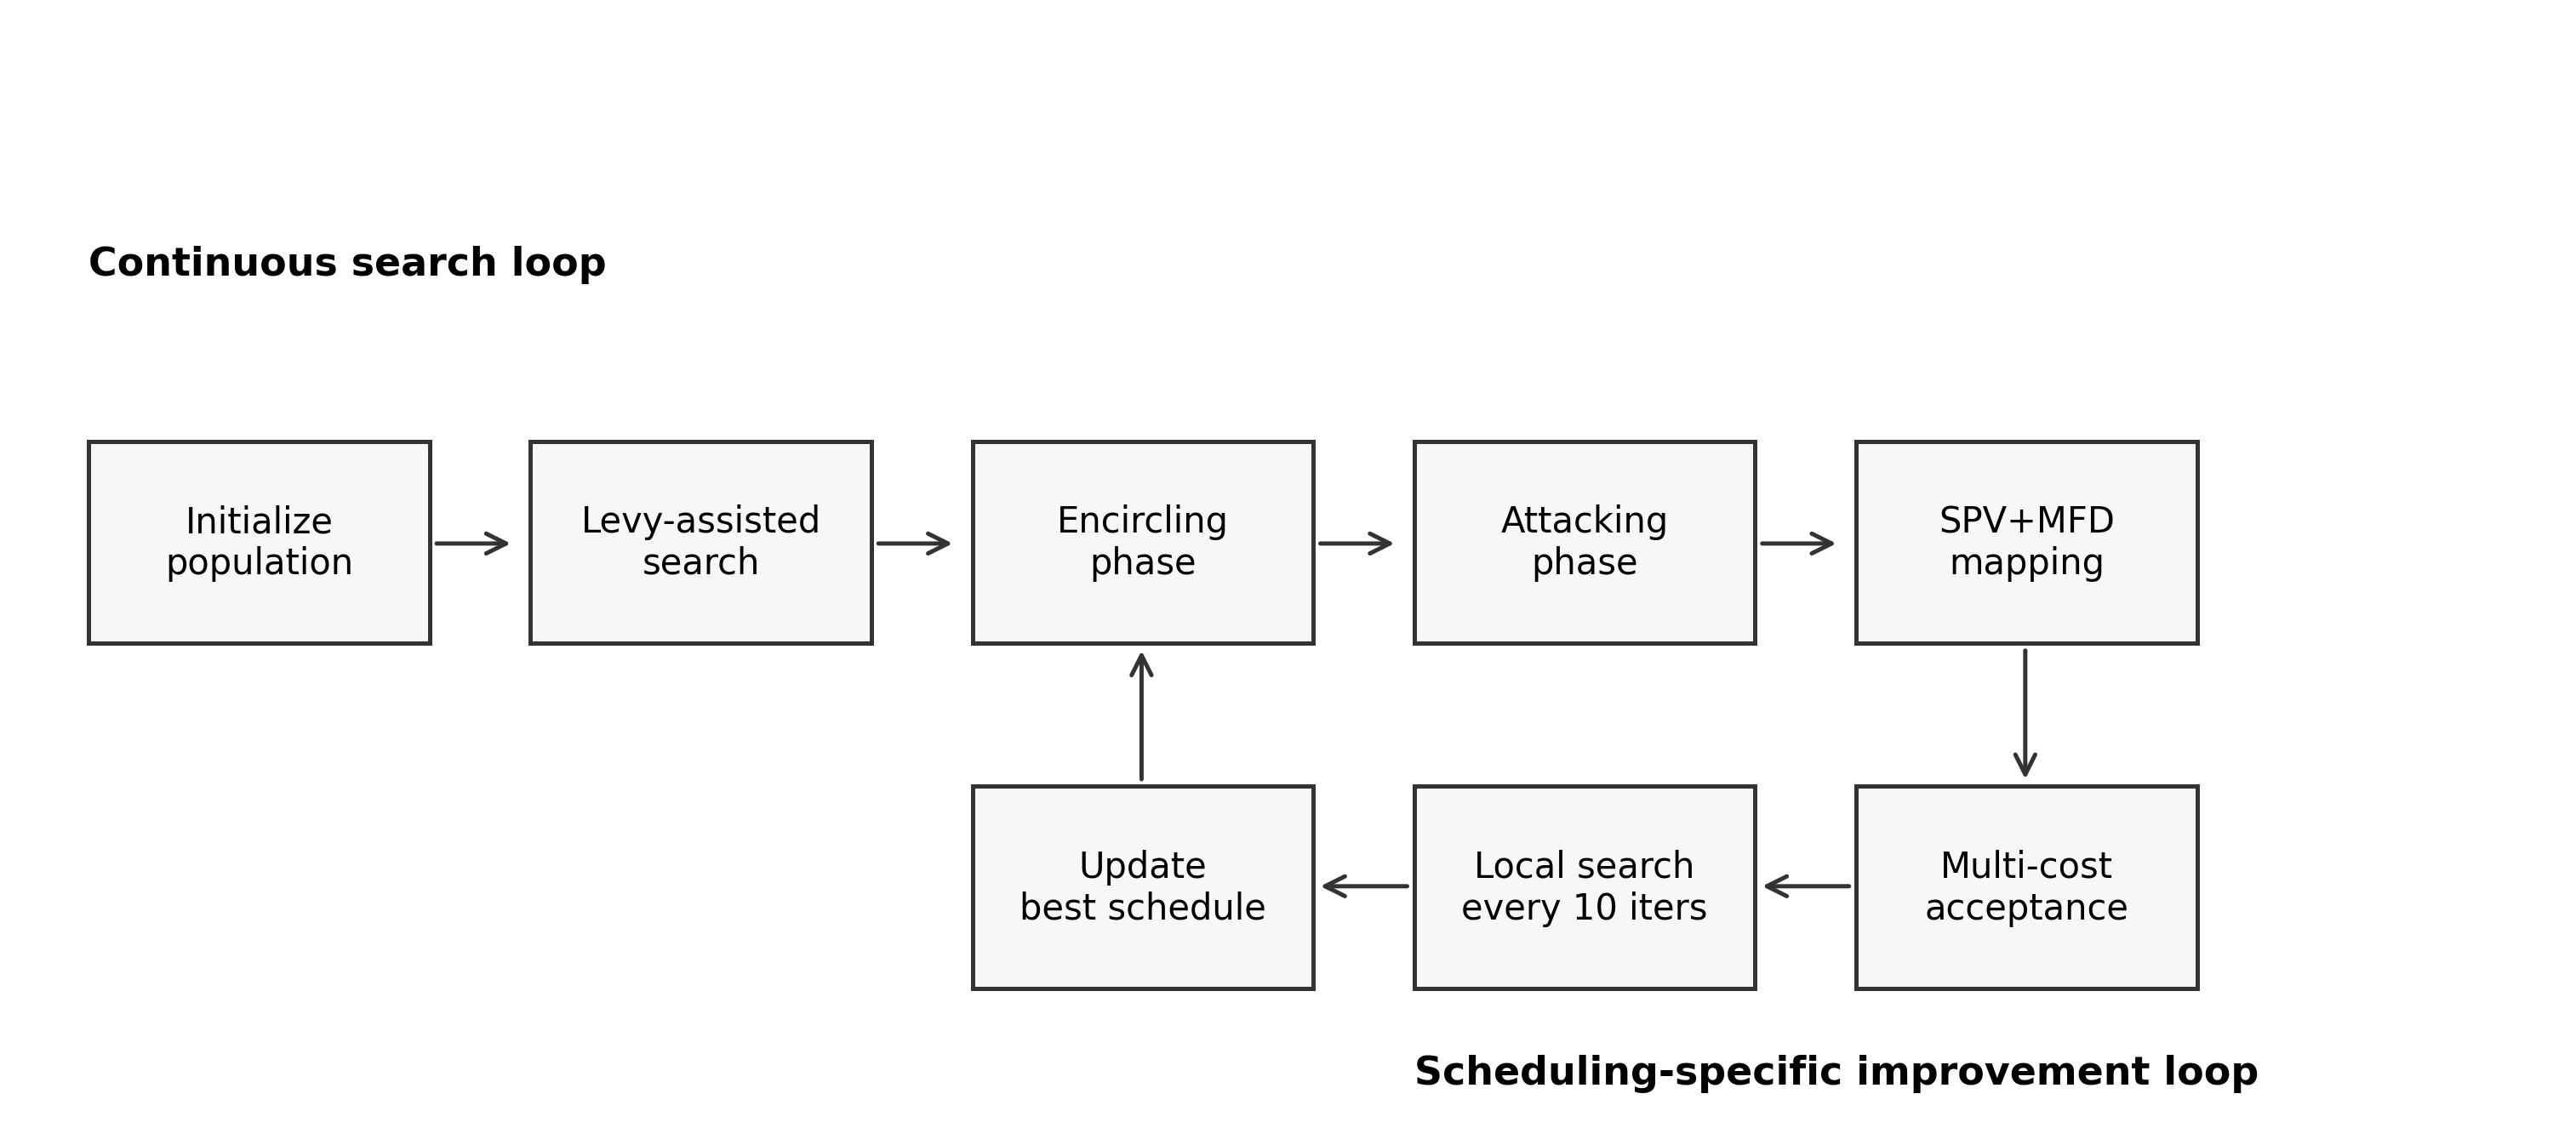
\includegraphics[width=0.92\textwidth]{figures/fig_lscbo_workflow.png}
\caption{Workflow of the LSCBO scheduler. L\'{e}vy-assisted CBO explores continuous task-order vectors; SPV+MFD decoding converts each vector into a feasible schedule; the scalarized objective evaluates makespan, energy, cost, and load balance; and task-reassignment local search periodically improves the current best assignment.}\label{fig:lscbo_workflow}
\end{figure}

\begin{algorithm}[ht]
\caption{LSCBO: Coyote-Badger Optimization with Task-Reassignment Local Search and L\'{e}vy Perturbation}\label{alg:lscbo}
\begin{algorithmic}[1]
\State \textbf{Input:} Population size $2P$, max iterations $T$, local search interval $I_{LS}$, L\'{e}vy parameter $\beta=1.5$, step scale $\alpha_0=0.05$
\State Initialize coyote population $\{X_{coy,i}^0\}_{i=1}^{P}$ and badger population $\{X_{bad,i}^0\}_{i=1}^{P}$
\State Initialize prey positions $X_{prey,i}^{0}$ as the midpoint of each coyote--badger pair
\State Evaluate all individuals; record global best solution $X^*$
\For{$t = 1$ \textbf{to} $T$}
    \State $\alpha \leftarrow \alpha_0(1 - t/T)$ \Comment{Decreasing step size}
    \For{each symbiotic pair $i = 1$ \textbf{to} $P$}
        \State \textbf{Phase 1 -- L\'{e}vy Searching:} Update $X_{coy,i}^{t}$ and $X_{bad,i}^{t}$ using Mantegna L\'{e}vy steps
        \State Apply boundary projection; decode via SPV+MFD; greedy accept if improved
        \State \textbf{Phase 2 -- Encircling:} Apply rotation matrix $R_{p,q}(\theta)$
        \State Decode via SPV+MFD; greedy accept if improved
        \State \textbf{Phase 3 -- Attacking:} Update toward leaders $\Omega_{coy}^{t}$, $\Omega_{bad}^{t}$
        \State Decode via SPV+MFD; greedy accept if improved
    \EndFor
    \If{$t \bmod I_{LS} = 0$}
        \State \textbf{Task-Reassignment Local Search:} Apply greedy task reassignment to $X^*$ (Section~\ref{sec:local_search})
        \State Update $X^*$ if improved
    \EndIf
    \State Update global leaders $\Omega_{coy}^{t}$, $\Omega_{bad}^{t}$
\EndFor
\State \textbf{Output:} Best schedule $X^*$
\end{algorithmic}
\end{algorithm}

\subsubsection{Population Initialization}
In the CBO framework, the population is modeled on the symbiotic relationship between coyotes and badgers. Let the total population be $2P$ individuals, partitioned into $P$ symbiotic pairs. For a $\Lambda$-dimensional search space, the initial positions of the $i$-th coyote and badger are sampled component-wise within $[\text{LB}, \text{UB}]$:
\begin{equation}
X_{coy, i}^{0} = \text{LB} + r_{coy,i}^{(0)} \odot (\text{UB} - \text{LB}), \quad r_{coy,i}^{(0)} \sim \mathcal{U}([0,1]^{\Lambda})
\end{equation}
\begin{equation}
X_{bad, i}^{0} = \text{LB} + r_{bad,i}^{(0)} \odot (\text{UB} - \text{LB}), \quad r_{bad,i}^{(0)} \sim \mathcal{U}([0,1]^{\Lambda})
\end{equation}
The target prey position for each pair is the midpoint:
\begin{equation}
X_{prey, i}^{0} = \frac{X_{coy, i}^{0} + X_{bad, i}^{0}}{2}
\end{equation}

\subsubsection{Phase 1: L\'{e}vy-Flight Searching}
The original CBO searching phase uses a tanh-based deterministic operator. LSCBO replaces this with L\'{e}vy-flight exploration, which introduces heavy-tailed stochastic perturbations:
\begin{equation}
X_{coy, i}^{t+1/3} = X_{coy, i}^t + \alpha \odot L_{coy,i}^{t}(\beta)
\end{equation}
\begin{equation}
X_{bad, i}^{t+1/3} = X_{bad, i}^t + \alpha \odot L_{bad,i}^{t}(\beta)
\end{equation}
where $\alpha = \alpha_0(1 - t/T)$ with $\alpha_0 = 0.05$ is a linearly decreasing step size, and $L(\beta)$ are L\'{e}vy-flight step vectors generated by the Mantegna scheme~\cite{Mantegna1994} with stability parameter $\beta = 1.5$. For each dimension $d$:
\begin{equation}
\ell_{i,d} = \frac{u_{i,d}}{|v_{i,d}|^{1/\beta}}, \quad u_{i,d}\sim\mathcal{N}(0,\sigma_u^2), \quad v_{i,d}\sim\mathcal{N}(0,1)
\end{equation}
\begin{equation}
\sigma_u = \left[\frac{\Gamma(1+\beta)\sin(\pi\beta/2)}{\Gamma((1+\beta)/2)\beta 2^{(\beta-1)/2}}\right]^{1/\beta}
\end{equation}
The L\'{e}vy distribution exhibits heavy-tailed power-law decay $L(s) \sim |s|^{-1-\beta}$, enabling occasional long-range jumps that enhance global exploration. The linearly decreasing $\alpha$ ensures that exploration is gradually reduced as the search progresses, allowing later iterations to focus on exploitation.

\subsubsection{Phase 2: Encircling}
Phase 2 of CBO is preserved unchanged. Individuals adjust their approach angles using a Givens-type rotation matrix acting on a randomly selected coordinate pair $(p,q)$:
\begin{equation}
\tilde{X}_{i}^{\,rot} = X_{prey, i}^{t} + R_{p,q}(\theta)\left(X_i^t - X_{prey, i}^{t}\right)
\end{equation}
where $R_{p,q}(\theta)$ is the identity matrix except for a $2\times2$ rotation block, and $\theta$ decreases linearly from $\theta_0 = \pi$ to zero. A greedy selection rule retains improved candidates.

\subsubsection{Phase 3: Static Attacking}
Phase 3 of CBO is preserved unchanged. Individuals are updated toward the current best coyote and badger leaders $\Omega_{coy}^{t}$ and $\Omega_{bad}^{t}$:
\begin{equation}
X_{coy, i}^{t+1} = X_{coy, i}^t + 0.5 \times (\Omega_{coy}^{t} - X_{coy, i}^t)
\end{equation}
\begin{equation}
X_{bad, i}^{t+1} = X_{bad, i}^t + 0.5 \times (\Omega_{bad}^{t} - X_{bad, i}^t)
\end{equation}
The fixed attack weight $w=0.5$ is preserved from the original CBO design so that LSCBO modifies the search framework only through the stated L\'{e}vy-assisted search and task-reassignment local search mechanisms.

\subsubsection{Task-Reassignment Local Search}\label{sec:local_search}
Every $I_{LS}=10$ iterations, LSCBO applies a greedy task-reassignment local search to the current global best solution. The procedure is:
\begin{enumerate}
    \item Identify the most-loaded VM ($VM_{worst}$) and the least-loaded VM ($VM_{best}$) based on current completion times.
    \item For each task $i$ currently assigned to $VM_{worst}$, compute the scalarized objective of the candidate schedule obtained by reassigning $i$ to $VM_{best}$.
    \item Accept the reassignment that maximally reduces the scalarized objective.
    \item Repeat up to $\min(10, \text{tasks on } VM_{worst})$ swaps per call.
\end{enumerate}

This local search directly exploits the scheduling problem structure---a design principle aligned with memetic algorithms~\cite{Moscato1989}. The operator performs greedy load balancing by redistributing tasks from over-utilized VMs to under-utilized VMs before execution. Candidate reassignments are accepted only if they improve the complete scalarized objective $F$ (not makespan alone), ensuring balanced optimization across all criteria used by the scheduler.

After every update, each coordinate is projected back to the feasible interval via $X_{i,d}^{t+1} \leftarrow \min(UB_d, \max(LB_d, X_{i,d}^{t+1}))$. For cloud scheduling, the projected vector is decoded via SPV+MFD and evaluated through the scalarized objective (Section~\ref{sec4}); the new position is greedily accepted only if it improves the current objective value.

\subsubsection{Evolution-Path Analysis}\label{sec:evolution}
To isolate the contribution of each design decision, we conducted a 5-stage evolution-path experiment (750 total trials, 5 stages $\times$ 5 task scales $\times$ 30 seeds) tracing the development from CBO to the local-search-enhanced variant. Table~\ref{tab:evolution} reports both makespan and the scalarized objective, because the scheduler accepts candidate solutions using the complete multi-cost score rather than makespan alone.

\begin{table}[ht]
\centering
\caption{Evolution Path from CBO to LSCBO (30 seeds, all task scales)}\label{tab:evolution}
\begin{tabular}{l c c c}
\toprule
\textbf{Stage} & \textbf{Makespan} & \textbf{Objective} & \textbf{Objective change} \\
\midrule
V1: CBO & 618.0 & 1.659 & --- \\
V2: CBO + L\'{e}vy & 615.4 & 1.651 & +0.5\% \\
V3: CBO + local search & 533.0 & 1.397 & +15.4\% \\
V4: CBO + L\'{e}vy + local search & 534.1 & 1.401 & $-0.3\%$ \\
\textbf{V5: final LSCBO} & \textbf{534.4} & \textbf{1.394} & \textbf{---} \\
\bottomrule
\end{tabular}
\smallskip

\footnotesize{Note: Objective change is computed against the preceding row, where positive values indicate improvement. The largest within-path improvement occurs when task-reassignment local search is introduced. Stages V4 and V5 use the identical final LSCBO configuration (CBO with L\'{e}vy-assisted search and task-reassignment local search); V5 is a confirmatory repeat, so its objective-change entry is shown as ``---'' because no design change is introduced relative to V4, and the small numerical V4$\rightarrow$V5 difference reflects only stochastic run-to-run variation.}
\end{table}

The evolution-path analysis shows that the largest improvement occurs when task-reassignment local search is introduced (V2$\rightarrow$V3, +15.4\% in objective). L\'{e}vy flight alone provides only a small improvement in this diagnostic path, and adding L\'{e}vy to an already local-search-enhanced variant does not consistently improve the scalarized objective. The final LSCBO design is therefore interpreted as a CBO-based scheduler whose main scheduling-specific mechanism is task reassignment, with L\'{e}vy perturbation retained as an auxiliary diversity mechanism rather than as the primary source of improvement.

\subsection{LSCBO-Based Cloud Task Scheduling}\label{sec:lscbo_scheduling}
Deploying LSCBO as a cloud task scheduler couples its continuous search with the multi-cost scheduling model and the SPV+MFD decoding introduced earlier in this section. At every iteration, each candidate position vector is decoded into a feasible task-to-VM assignment, scored by the scalarized multi-cost objective, and accepted greedily when it improves the incumbent; every $I_{LS}$ iterations the task-reassignment local search refines the current best schedule. Figure~\ref{fig:lscbo_workflow} summarizes this end-to-end pipeline and Algorithm~\ref{alg:lscbo} states the complete procedure.

\subsubsection{Computational Complexity}
Let $S=2P$ denote the total number of search agents, $D$ the continuous search dimension, $T$ the maximum number of iterations, $N$ the number of tasks, and $M$ the number of VMs. The three-phase per-iteration update requires $O(SD)$ operations per phase, yielding $O(TSD)$ overall for continuous benchmarks. For cloud scheduling, SPV+MFD decoding adds $O(N\log N + M)$ per candidate, giving $O(TS(N\log N + M))$ total under straightforward decoding. The task-reassignment local search is invoked every $I_{LS}=10$ iterations; each call evaluates at most $L=\min(10,n_{worst})$ reassignment candidates from the most-loaded VM. With direct recomputation, one local-search call costs $O(L(N+M))$, and the total local-search overhead is $O(\lfloor T/I_{LS}\rfloor L(N+M))$. In the CloudSim experiments this overhead is bounded by at most 20 additional schedule evaluations per run.

\section{Experimental Results}\label{sec5}

The performance of LSCBO is evaluated through two experimental series. Series~1 validates the algorithm's global optimization capability on 29 CEC2017 benchmark functions against six comparison algorithms. Series~2 evaluates LSCBO in the cloud task scheduling domain using a CloudSim Plus scheduling pipeline---in which every formal row is executed through a full CloudSim Plus simulation---against eight population-based meta-heuristic schedulers across comprehensive experimental campaigns.

To ensure a fair comparison, the comparison algorithms retain their standard control parameters where applicable, while population size, iteration count, task instances, VM instances, and random seeds are fixed within each experimental series. Table~\ref{tab:param_cec} summarizes the settings for the CEC2017 experiments (Series~1), and Table~\ref{tab:param_cloudsim} for the cloud scheduling experiments (Series~2).

\subsection{Experimental Series 1: CEC2017 Global Optimization Benchmarks}\label{sec:cec2017}

To validate LSCBO's fundamental optimization capability before applying it to the scheduling domain, we evaluate the algorithm on the CEC2017 benchmark suite, which comprises rotated and shifted test functions of varying complexity and modality. This two-tier evaluation strategy---benchmark validation followed by domain application---follows the established methodology in meta-heuristic research~\cite{Heidari2019,Mirjalili2016,Khatab2025}. This series is intended as a general-capability sanity check rather than as a novelty claim in continuous optimization: its purpose is to confirm that the L\'{e}vy-modified search does not degrade the base optimizer before the algorithm is applied to its primary target domain, cloud task scheduling. Achieving competitive (rather than uniquely dominant) continuous-optimization performance is sufficient for this purpose.

\subsubsection{CEC2017 Settings}
All CEC2017 experiments use a population size of 30 with 10,000 iterations (300,000 function evaluations per run), with $D=30$ and search bounds $[-100, 100]^D$. We selected 29 functions (F1, F3--F30; F2 is deprecated) from the CEC2017 suite~\cite{CEC2017}.

\begin{table}[ht]
\centering
\caption{Parameter Settings for CEC2017 Experiments (Series~1)}\label{tab:param_cec}
\begin{tabular}{l l l}
\toprule
\textbf{Algorithm} & \textbf{Parameter} & \textbf{Value} \\
\midrule
LSCBO & Population size & 30 \\
       & Iterations & 10,000 \\
       & L\'{e}vy stability $\beta$ & 1.5 \\
       & Step scale $\alpha_0$ & 0.05 \\
\midrule
CBO & Population size & 30 \\
    & Iterations & 10,000 \\
    & Rotation range $\theta_0$ & $\pi$ \\
    & Attack weight $w$ & 0.5 \\
\midrule
GTO & Population size & 30 \\
    & Migration rate $p$ & 0.03 \\
    & Silverback factor $\beta$ & 3.0 \\
\midrule
DE & Population size & 30 \\
    & Scale factor $F$ & 0.5 \\
    & Crossover rate $CR$ & 0.9 \\
\midrule
PSO & Population size & 30 \\
    & Inertia weight $w$ & $0.9 \rightarrow 0.4$ \\
    & Cognitive/social $c_1, c_2$ & 2.0, 2.0 \\
\midrule
SA & Initial temperature $T_0$ & 1,000 \\
    & Cooling rate $\gamma$ & 0.95 \\
\midrule
GWO & Population size & 30 \\
    & Convergence constant $a$ & $2 \rightarrow 0$ \\
\midrule
\multicolumn{3}{l}{\footnotesize{All algorithms: $D=30$, bounds $[-100,100]^D$, 30 independent runs per function.}} \\
\bottomrule
\end{tabular}
\end{table}

\subsubsection{CEC2017 Ranking Comparison}
We compare LSCBO against six algorithms on all 29 CEC2017 functions: CBO~\cite{Khatab2025}, GTO~\cite{Abdollahzadeh2021}, DE~\cite{Storn1997}, PSO~\cite{Kennedy1995}, SA~\cite{Kirkpatrick1983}, and GWO~\cite{Mirjalili2014}. This selection encompasses both classical and more recent optimizers, providing a balanced reference for convergence speed, solution quality, and stability under an identical evaluation budget. The two experimental series intentionally use different comparison sets: the CEC2017 series includes the standard continuous-optimization references DE and SA, which are conventional baselines for unconstrained numerical benchmarking, whereas the cloud-scheduling series (Section~\ref{sec:cloudsim_exp}) substitutes the recent population-based optimizers WOA, HHO, DBO, and AOA, which are the more representative meta-heuristic baselines in the cloud task-scheduling literature. The shared anchors CBO, GTO, PSO, and GWO appear in both series to maintain a consistent reference across the two settings. All algorithms are evaluated over 300,000 function evaluations (population size 30 $\times$ 10,000 iterations) per run, with $D=30$ and search bounds $[-100, 100]^D$. Table~\ref{tab:cec_ranking} presents the Friedman average ranking across all 29 functions, and Fig.~\ref{fig:cec_ranking} visualizes the same ranking.

\begin{table}[ht]
\centering
\caption{Friedman Ranking of Algorithms on CEC2017 (29 Functions, 30 Runs per Function)}\label{tab:cec_ranking}
\begin{tabular}{l c}
\toprule
\textbf{Algorithm} & \textbf{Average Rank} \\
\midrule
LSCBO          & 1.86 \\
GTO            & 1.90 \\
DE             & 2.28 \\
CBO            & 4.07 \\
PSO            & 5.10 \\
SA             & 5.93 \\
GWO            & 6.86 \\
\bottomrule
\end{tabular}
\end{table}

\begin{figure}[htbp]
\centering

\includegraphics[width=0.85\textwidth]{figures/fig1_cec_ranking.png}
\caption{Friedman average ranking of seven algorithms on 29 CEC2017 benchmark functions. LSCBO obtains the lowest average rank (1.86) within this comparison set, followed by GTO (1.90) and DE (2.28). The global Friedman test confirms significant differences ($\chi^2 = 156.04$, $p < 0.0001$).}\label{fig:cec_ranking}
\end{figure}

\textbf{Statistical Analysis.} A Friedman test over the 29 CEC2017 functions (functions as blocks, algorithms as treatments) confirms significant differences among algorithms ($\chi^2 = 156.04$, $p < 0.0001$). Post-hoc Nemenyi analysis~\cite{Demsar2006} yields a critical difference $\mathrm{CD} = 1.673$ at $\alpha = 0.05$. LSCBO, GTO, and DE form the top cluster with pairwise rank gaps within the CD, indicating competitive continuous search performance among these three algorithms. Pairwise conclusions are further examined with Wilcoxon signed-rank tests~\cite{Wilcoxon1945}. LSCBO achieves statistically significant wins over CBO, PSO, SA, and GWO ($p < 0.001$ for each), and statistical parity with DE ($p = 0.059$) and GTO ($p = 0.481$). It should be noted that the comparison set does not include specialized continuous solvers such as L-SHADE~\cite{Tanabe2014} or CMA-ES~\cite{Hansen2001}, and the primary evaluation target of LSCBO is discrete cloud scheduling (Section~\ref{sec:cloudsim_exp}). Per-function average fitness values and standard deviations for all algorithms are available in the Supplementary Materials.

\subsubsection{Convergence Analysis on CEC2017}
Convergence curves on representative CEC2017 functions demonstrate that LSCBO exhibits rapid early convergence and continues to improve in later iterations. The algorithm reaches highly competitive final fitness values compared with the tested baselines. Complete per-function convergence data is available in the Supplementary Materials and project repository.

\subsection{Experimental Series 2: Cloud Task Scheduling}\label{sec:cloudsim_exp}

\subsubsection{CloudSim Settings}
All cloud-scheduling meta-heuristic experiments use a population size of 20 with 20 iterations, corresponding to 20 initial evaluations and 400 iteration evaluations per run. This compact budget reflects the time-constrained nature of batch scheduling decisions, where each candidate evaluation entails a full schedule decoding and cost computation; it is applied identically to all compared schedulers so that the comparison remains fair under a common evaluation budget. Because every scheduler operates under the same modest iteration count, the reported differences characterize the proposed CBO-plus-local-search design pattern within this shared protocol rather than asymptotic search behavior under very large budgets, which is left to future work. For LSCBO, the local search invoked every $I_{LS}=10$ iterations performs at most 10 greedy task-reassignment attempts per call. These local-search attempts are counted separately: the worst-case LSCBO budget is therefore 440 total schedule evaluations including initialization, compared with 420 for the other schedulers. This approximately 4.8\% overhead is reported explicitly rather than treated as an identical evaluation budget.

\begin{table}[ht]
\centering
\caption{Parameter Settings for CloudSim Experiments (Series~2)}\label{tab:param_cloudsim}
\begin{tabular}{l l l}
\toprule
\textbf{Algorithm} & \textbf{Parameter} & \textbf{Value} \\
\midrule
LSCBO & Population size & 20 \\
       & Iterations & 20 \\
       & L\'{e}vy stability $\beta$ & 1.5 \\
       & Step scale $\alpha_0$ & 0.05 \\
       & Local search interval $I_{LS}$ & 10 \\
       & Attack weight $w$ & 0.5 \\
\midrule
CBO & Population size & 20 \\
    & Iterations & 20 \\
    & Rotation range $\theta_0$ & $\pi$ \\
    & Attack weight $w$ & 0.5 \\
\midrule
GTO & Population size & 20 \\
    & Iterations & 20 \\
    & Migration probability $p$ & 0.03 \\
\midrule
WOA, GWO & Population size & 20 \\
    & Iterations & 20 \\
    & Convergence constant $a$ & $2 \rightarrow 0$ \\
\midrule
HHO & Population size & 20 \\
    & Iterations & 20 \\
\midrule
PSO & Population size & 20 \\
    & Iterations & 20 \\
    & Inertia weight $w$ & $0.9 \rightarrow 0.4$ \\
    & Cognitive/social $c_1, c_2$ & 2.0, 2.0 \\
\midrule
DBO & Population size & 20 \\
    & Iterations & 20 \\
    & Guide probability $P_{percent}$ & 0.2 \\
\midrule
AOA & Population size & 20 \\
    & Iterations & 20 \\
    & Sensitive parameter $\alpha$ & 5.0 \\
\midrule
\multicolumn{3}{p{0.88\textwidth}}{\footnotesize{All CloudSim algorithms are evaluated on identical task instances, VM instances, seeds, population sizes, and iteration counts. LSCBO additionally reports the counted local-search overhead described above.}} \\
\bottomrule
\end{tabular}
\end{table}

\subsubsection{CloudSim Configuration}
The scheduling implementation is built around CloudSim Plus 8.0.0~\cite{Calheiros2011,SilvaFilho2017}. The simulated environment comprises one datacenter with at least 10 hosts; each host has 4 CPU cores, 16 GB RAM, 1 TB storage, and 10 Gbps bandwidth, and the host count is expanded when needed to allocate all VMs. TimeShared policies are used for both hosts and VMs. All experiments use $M=50$ heterogeneous VMs (MIPS 500--2000, uniformly sampled), task MI ranging from 1000 to 20000 (uniformly sampled), and deterministic seeds 43--72 for reproducibility (30 independent runs). The full formal comparison contains 12,780 multi-cost scheduling rows generated from this task/VM model. Every one of these 12,780 rows was additionally executed through a full CloudSim Plus simulation: all scheduled cloudlets completed successfully (12,780/12,780 rows validated), and the CloudSim-measured makespan tracks the analytic multi-cost values reported in this section closely, confirming that the reported schedules are executable and faithfully simulated rather than only analytically scored. The complete implementation is publicly available at \url{https://github.com/Lazywords2006/LSCBO}.

\subsubsection{Main Comparison of Meta-Heuristic Schedulers}
Table~\ref{tab:main_makespan} presents the makespan comparison across five task scales. All values are the mean of 30 independent runs under fixed seeds (43--72).

\begin{table*}[ht]
\centering
\caption{Cross-Scale Makespan Comparison (mean, 30 runs per scale)}\label{tab:main_makespan}
\resizebox{\textwidth}{!}{
\begin{tabular}{l c c c c c}
\toprule
\textbf{Algorithm} & \textbf{$N=200$} & \textbf{$N=500$} & \textbf{$N=1000$} & \textbf{$N=2000$} & \textbf{$N=5000$} \\
\midrule
\textbf{LSCBO} & \textbf{46.9} & \textbf{121.4} & \textbf{275.7} & \textbf{601.3} & \textbf{1620.5} \\
WOA & 67.8 & 171.1 & 342.8 & 699.9 & 1794.1 \\
HHO & 67.1 & 172.0 & 344.7 & 701.6 & 1785.8 \\
CBO (baseline) & 67.0 & 171.2 & 344.6 & 705.0 & 1792.6 \\
PSO & 68.5 & 170.3 & 344.1 & 703.1 & 1798.5 \\
DBO & 67.7 & 171.9 & 345.6 & 701.1 & 1797.9 \\
GTO & 68.5 & 170.6 & 347.3 & 702.2 & 1790.6 \\
GWO & 68.7 & 171.7 & 347.0 & 702.0 & 1800.3 \\
AOA & 68.5 & 172.2 & 345.6 & 702.0 & 1803.1 \\
\bottomrule
\end{tabular}
}
\end{table*}

Table~\ref{tab:main_lbr} presents the load-balance ratio (LBR, lower is better).

\begin{table*}[ht]
\centering
\caption{Cross-Scale Load-Balance Ratio (LBR) Comparison}\label{tab:main_lbr}
\resizebox{\textwidth}{!}{
\begin{tabular}{l c c c c c}
\toprule
\textbf{Algorithm} & \textbf{$N=200$} & \textbf{$N=500$} & \textbf{$N=1000$} & \textbf{$N=2000$} & \textbf{$N=5000$} \\
\midrule
\textbf{LSCBO} & \textbf{1.359} & \textbf{1.355} & \textbf{1.492} & \textbf{1.597} & \textbf{1.709} \\
WOA & 1.821 & 1.797 & 1.799 & 1.827 & 1.875 \\
HHO & 1.800 & 1.806 & 1.804 & 1.832 & 1.867 \\
CBO & 1.798 & 1.799 & 1.804 & 1.838 & 1.874 \\
PSO & 1.834 & 1.789 & 1.803 & 1.832 & 1.879 \\
DBO & 1.819 & 1.808 & 1.809 & 1.827 & 1.878 \\
GTO & 1.838 & 1.796 & 1.820 & 1.834 & 1.874 \\
GWO & 1.842 & 1.802 & 1.817 & 1.831 & 1.882 \\
AOA & 1.836 & 1.810 & 1.810 & 1.831 & 1.885 \\
\bottomrule
\end{tabular}
}
\end{table*}

Across the 30-seed formal comparison, LSCBO achieves the lowest mean makespan and LBR at all five task scales. Table~\ref{tab:per_scale_cbo} reports the corresponding multi-cost improvements over the standardized CBO baseline. The improvement is largest at smaller task scales and remains positive at $N=5000$, where the search space is larger and the relative gap naturally narrows.

\begin{table}[ht]
\centering
\caption{Per-Scale LSCBO Improvement over CBO by Cost Component}\label{tab:per_scale_cbo}
\begin{tabular}{l c c c c c}
\toprule
\textbf{Scale} & \textbf{Makespan} & \textbf{Energy} & \textbf{Cost} & \textbf{LBR} & \textbf{Objective} \\
\midrule
$N=200$  & 30.1\% & 24.1\% & 2.9\% & 24.4\% & 22.6\% \\
$N=500$  & 29.1\% & 22.9\% & 2.3\% & 24.7\% & 22.0\% \\
$N=1000$ & 20.0\% & 15.5\% & 1.3\% & 17.3\% & 15.1\% \\
$N=2000$ & 14.7\% & 11.3\% & 0.7\% & 13.1\% & 11.2\% \\
$N=5000$ & 9.6\%  & 7.3\%  & 0.4\% & 8.8\%  & 7.4\% \\
\bottomrule
\end{tabular}
\end{table}

\begin{figure*}[htbp]
\centering
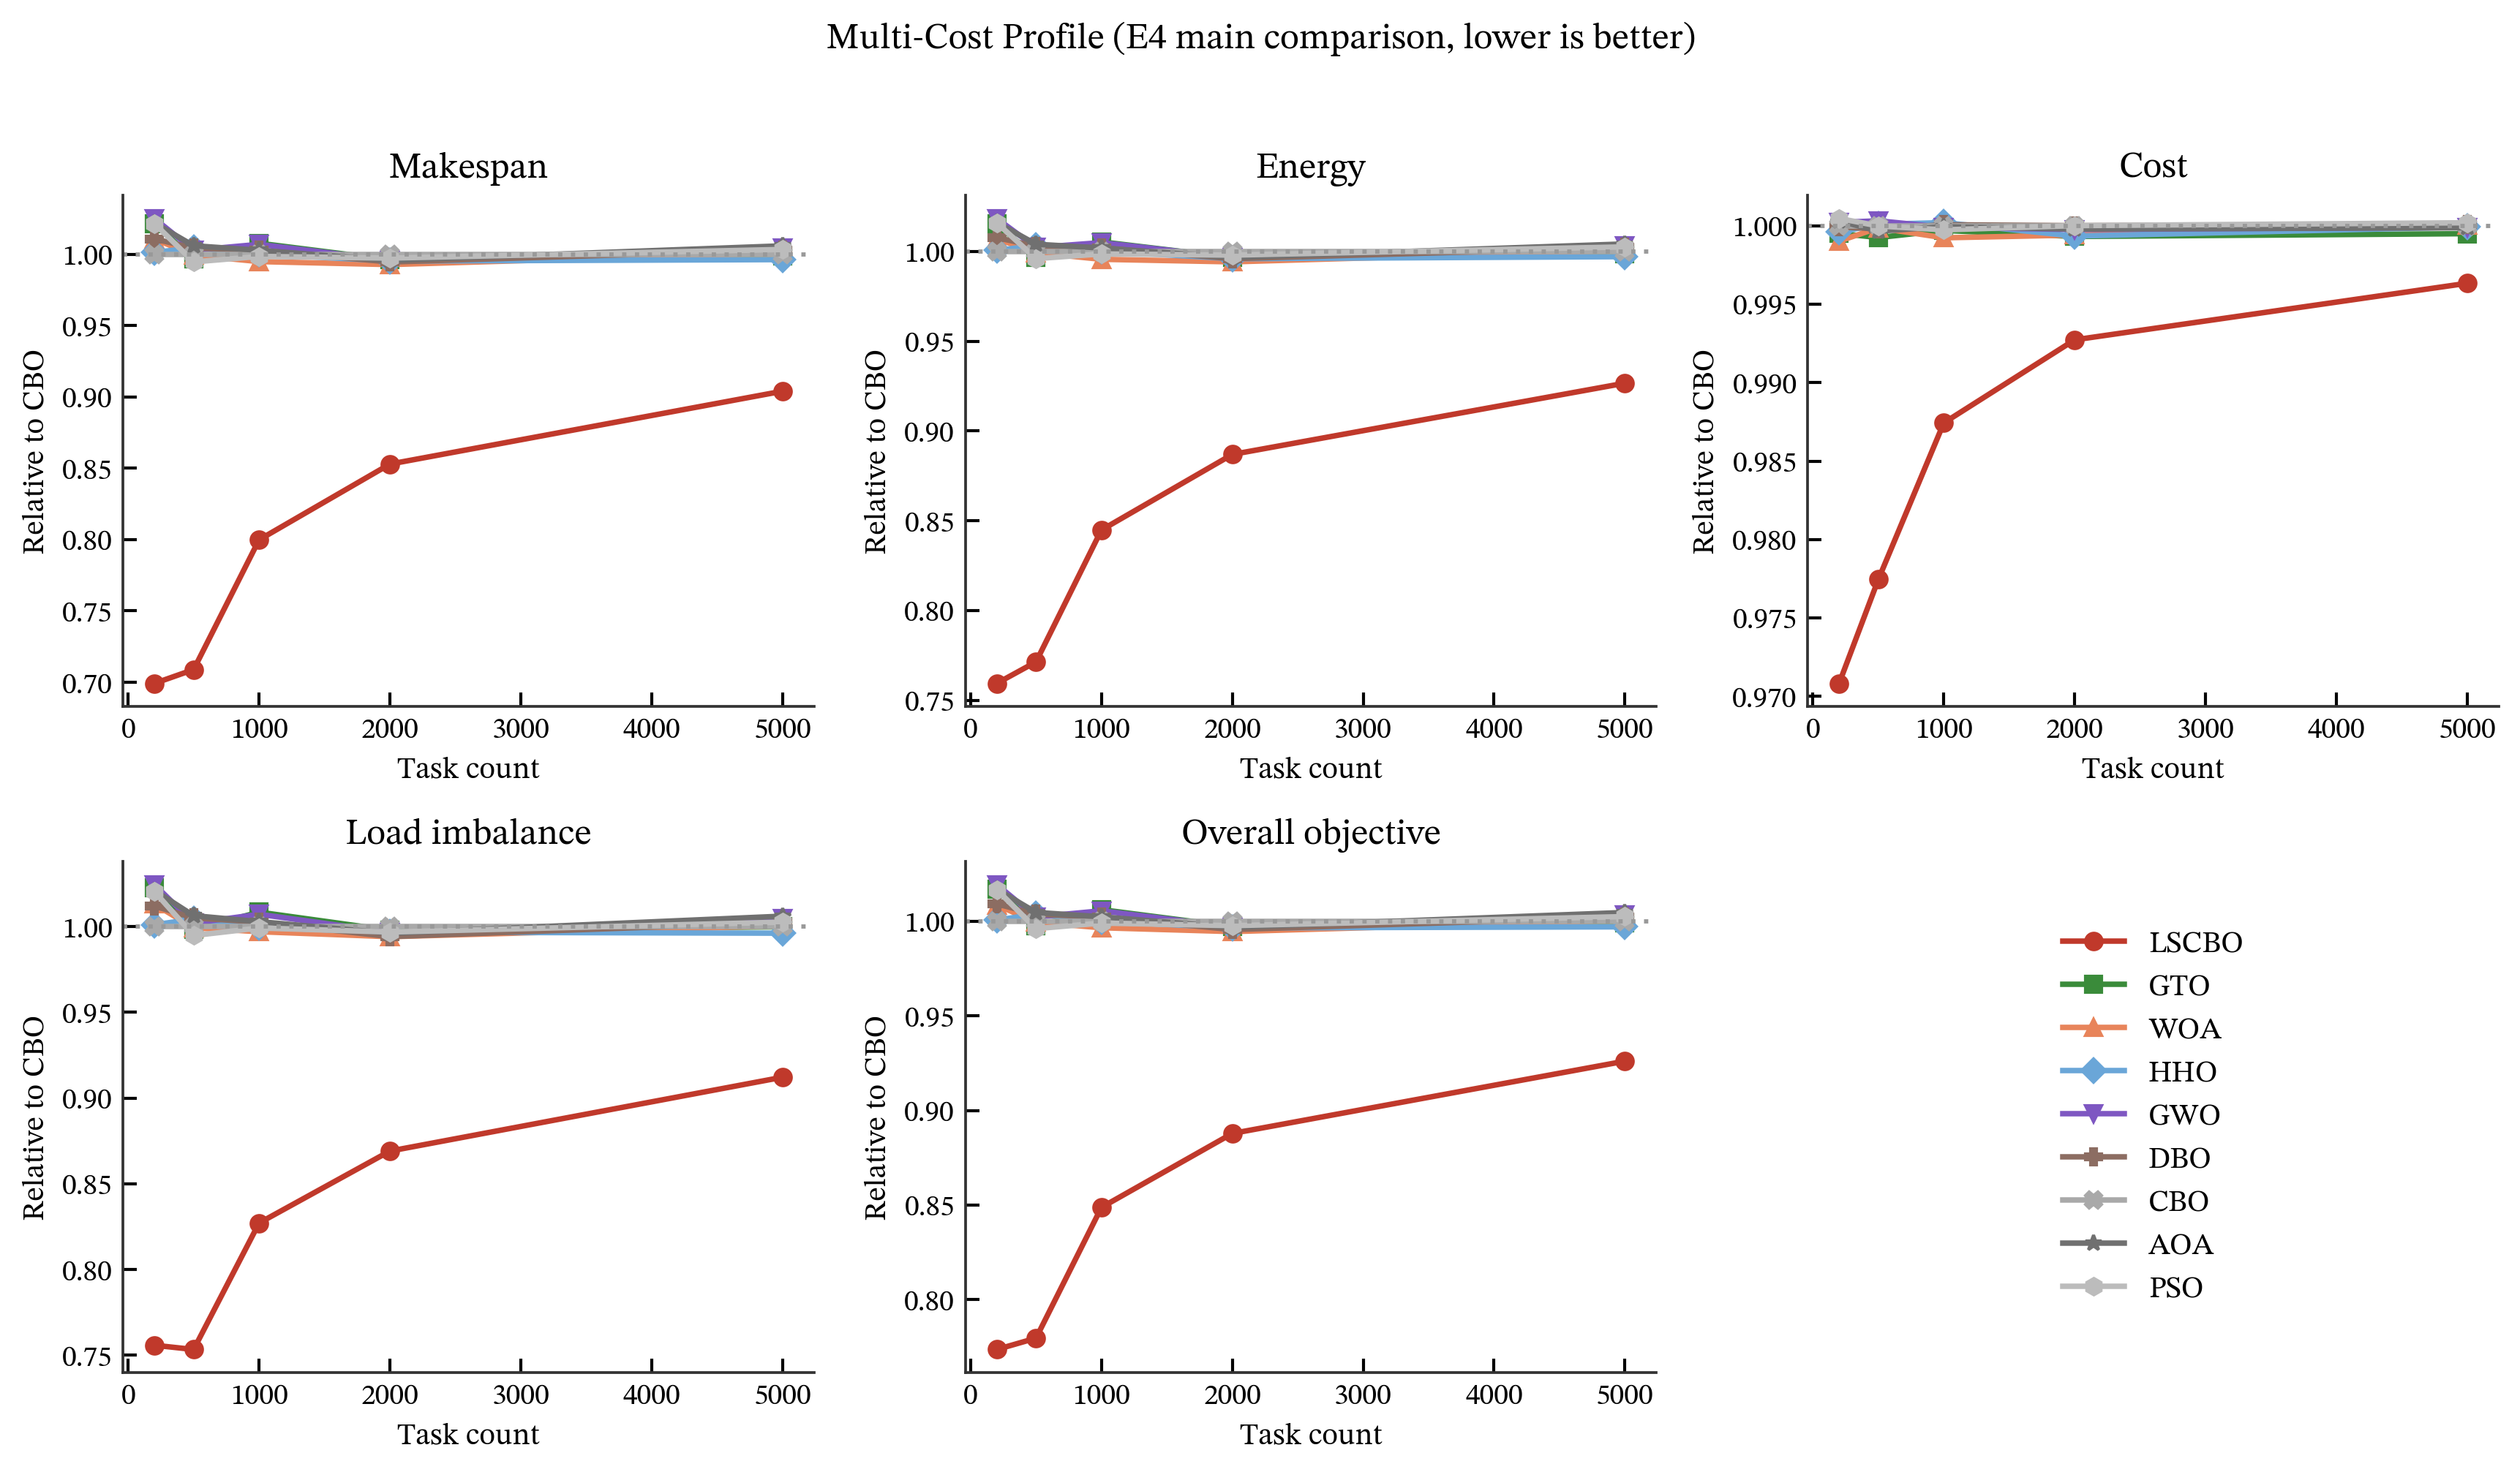
\includegraphics[width=0.95\textwidth]{figures/fig_claim_multicost_profile.png}
\caption{Formal multi-cost profile aligned with the E4 main-comparison setup. The figure uses the SPV+MFD decoding, power/cost parameters, five task scales, nine algorithms, and 30 paired seeds; each panel reports the mean value relative to CBO at the same task scale, where values below 1.0 indicate improvement over the standardized CBO baseline.}\label{fig:multicost_profile}
\end{figure*}

Figure~\ref{fig:multicost_profile} complements the makespan and LBR tables by exposing the cost components used by the scalarized objective. It shows that the strongest effects appear in makespan, energy, and load balance, while cost improves more modestly because all methods execute the same task set on the same VM-price model. This connects the algorithmic acceptance rule with the cloud-scheduling model in Section~\ref{sec4}.

\subsubsection{Convergence Analysis}\label{sec:convergence}
Representative convergence traces are used as a diagnostic view of search behavior rather than as the primary statistical evidence. Figure~\ref{fig:convergence_trace} shows stored LSCBO scheduling traces across task scales ($N=100$ to $N=1000$) under a fixed seed, with each curve normalized to its own iteration-0 value to expose within-run improvement on a common scale. The traces illustrate how LSCBO's candidate quality evolves as the problem size grows under the same iteration budget; the comparative conclusion against the baselines is based on the paired repeated-run tables and Friedman/Wilcoxon tests rather than on a single trace.

\begin{figure}[htbp]
\centering
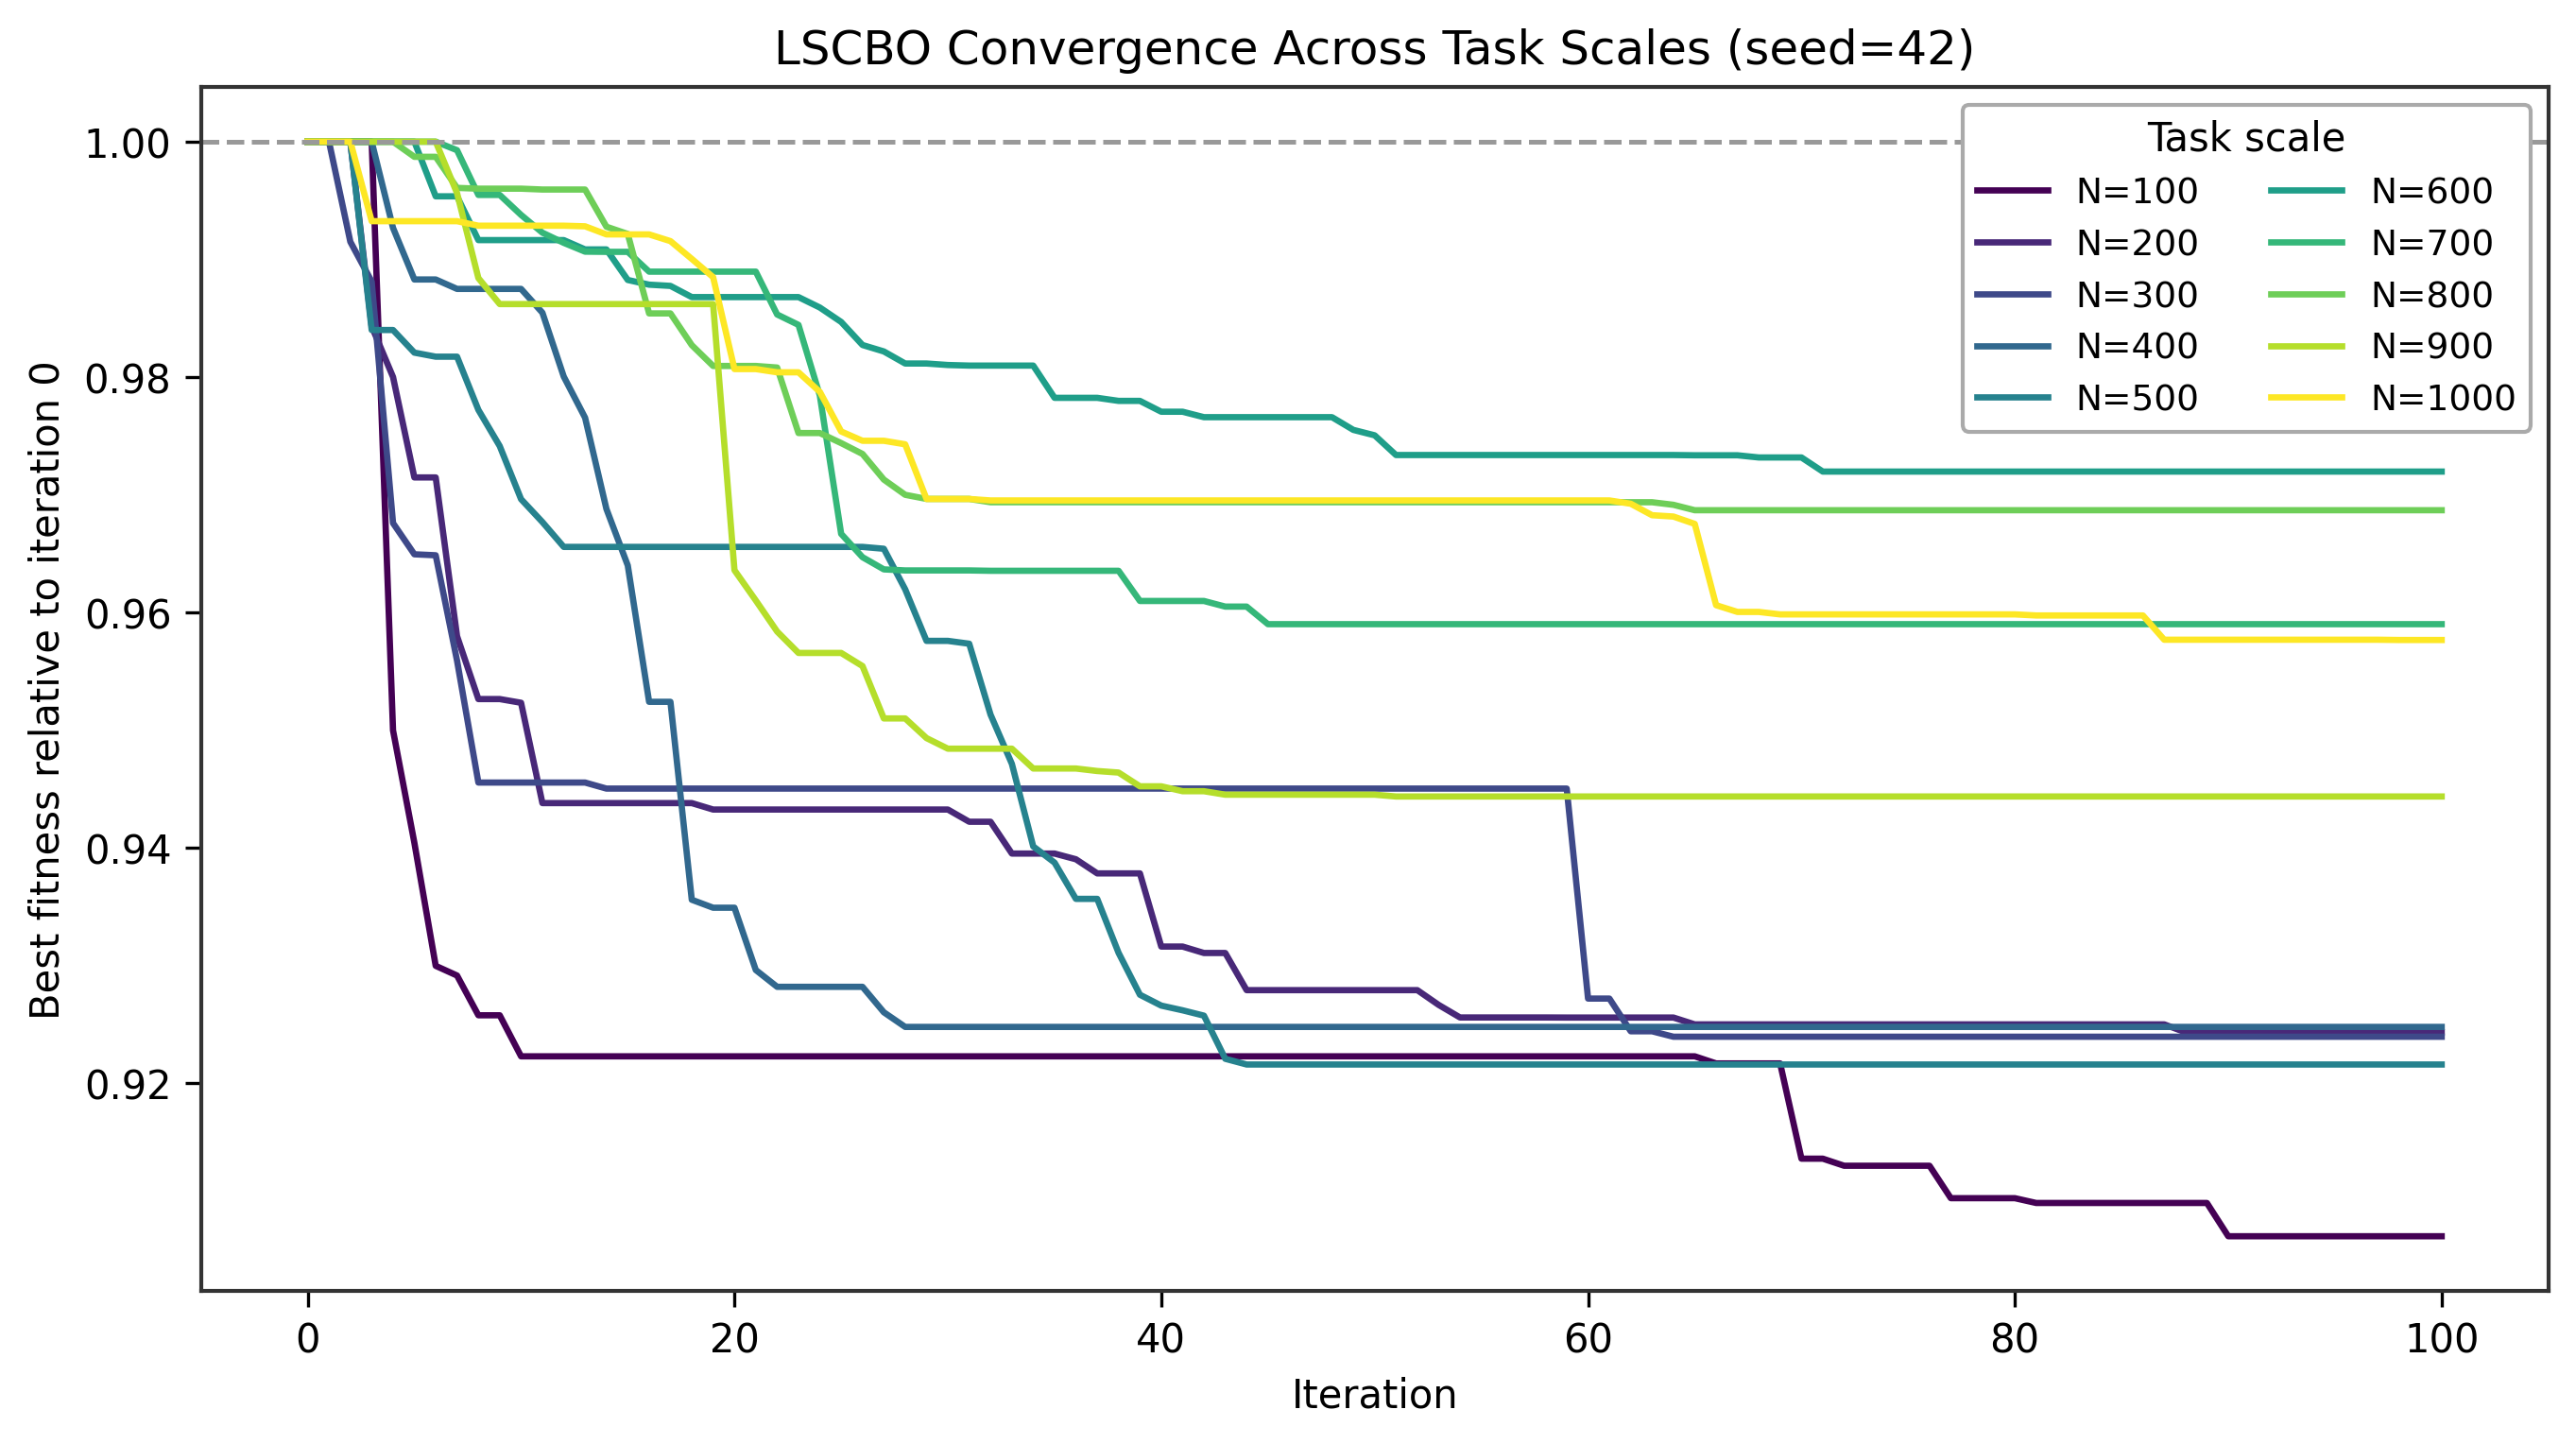
\includegraphics[width=0.85\textwidth]{figures/fig_lscbo_convergence_trace.png}
\caption{Diagnostic convergence traces of LSCBO across task scales ($N=100$--$1000$) under a fixed seed. Each curve is normalized by its own initial best fitness to show relative within-run improvement on a common scale; this figure is illustrative of LSCBO's search behavior and is not used as the primary statistical evidence, which comes from the paired repeated-run tables and Friedman/Wilcoxon tests.}\label{fig:convergence_trace}
\end{figure}

\subsubsection{Friedman Ranking and Statistical Tests}

\begin{figure}[htbp]
\centering
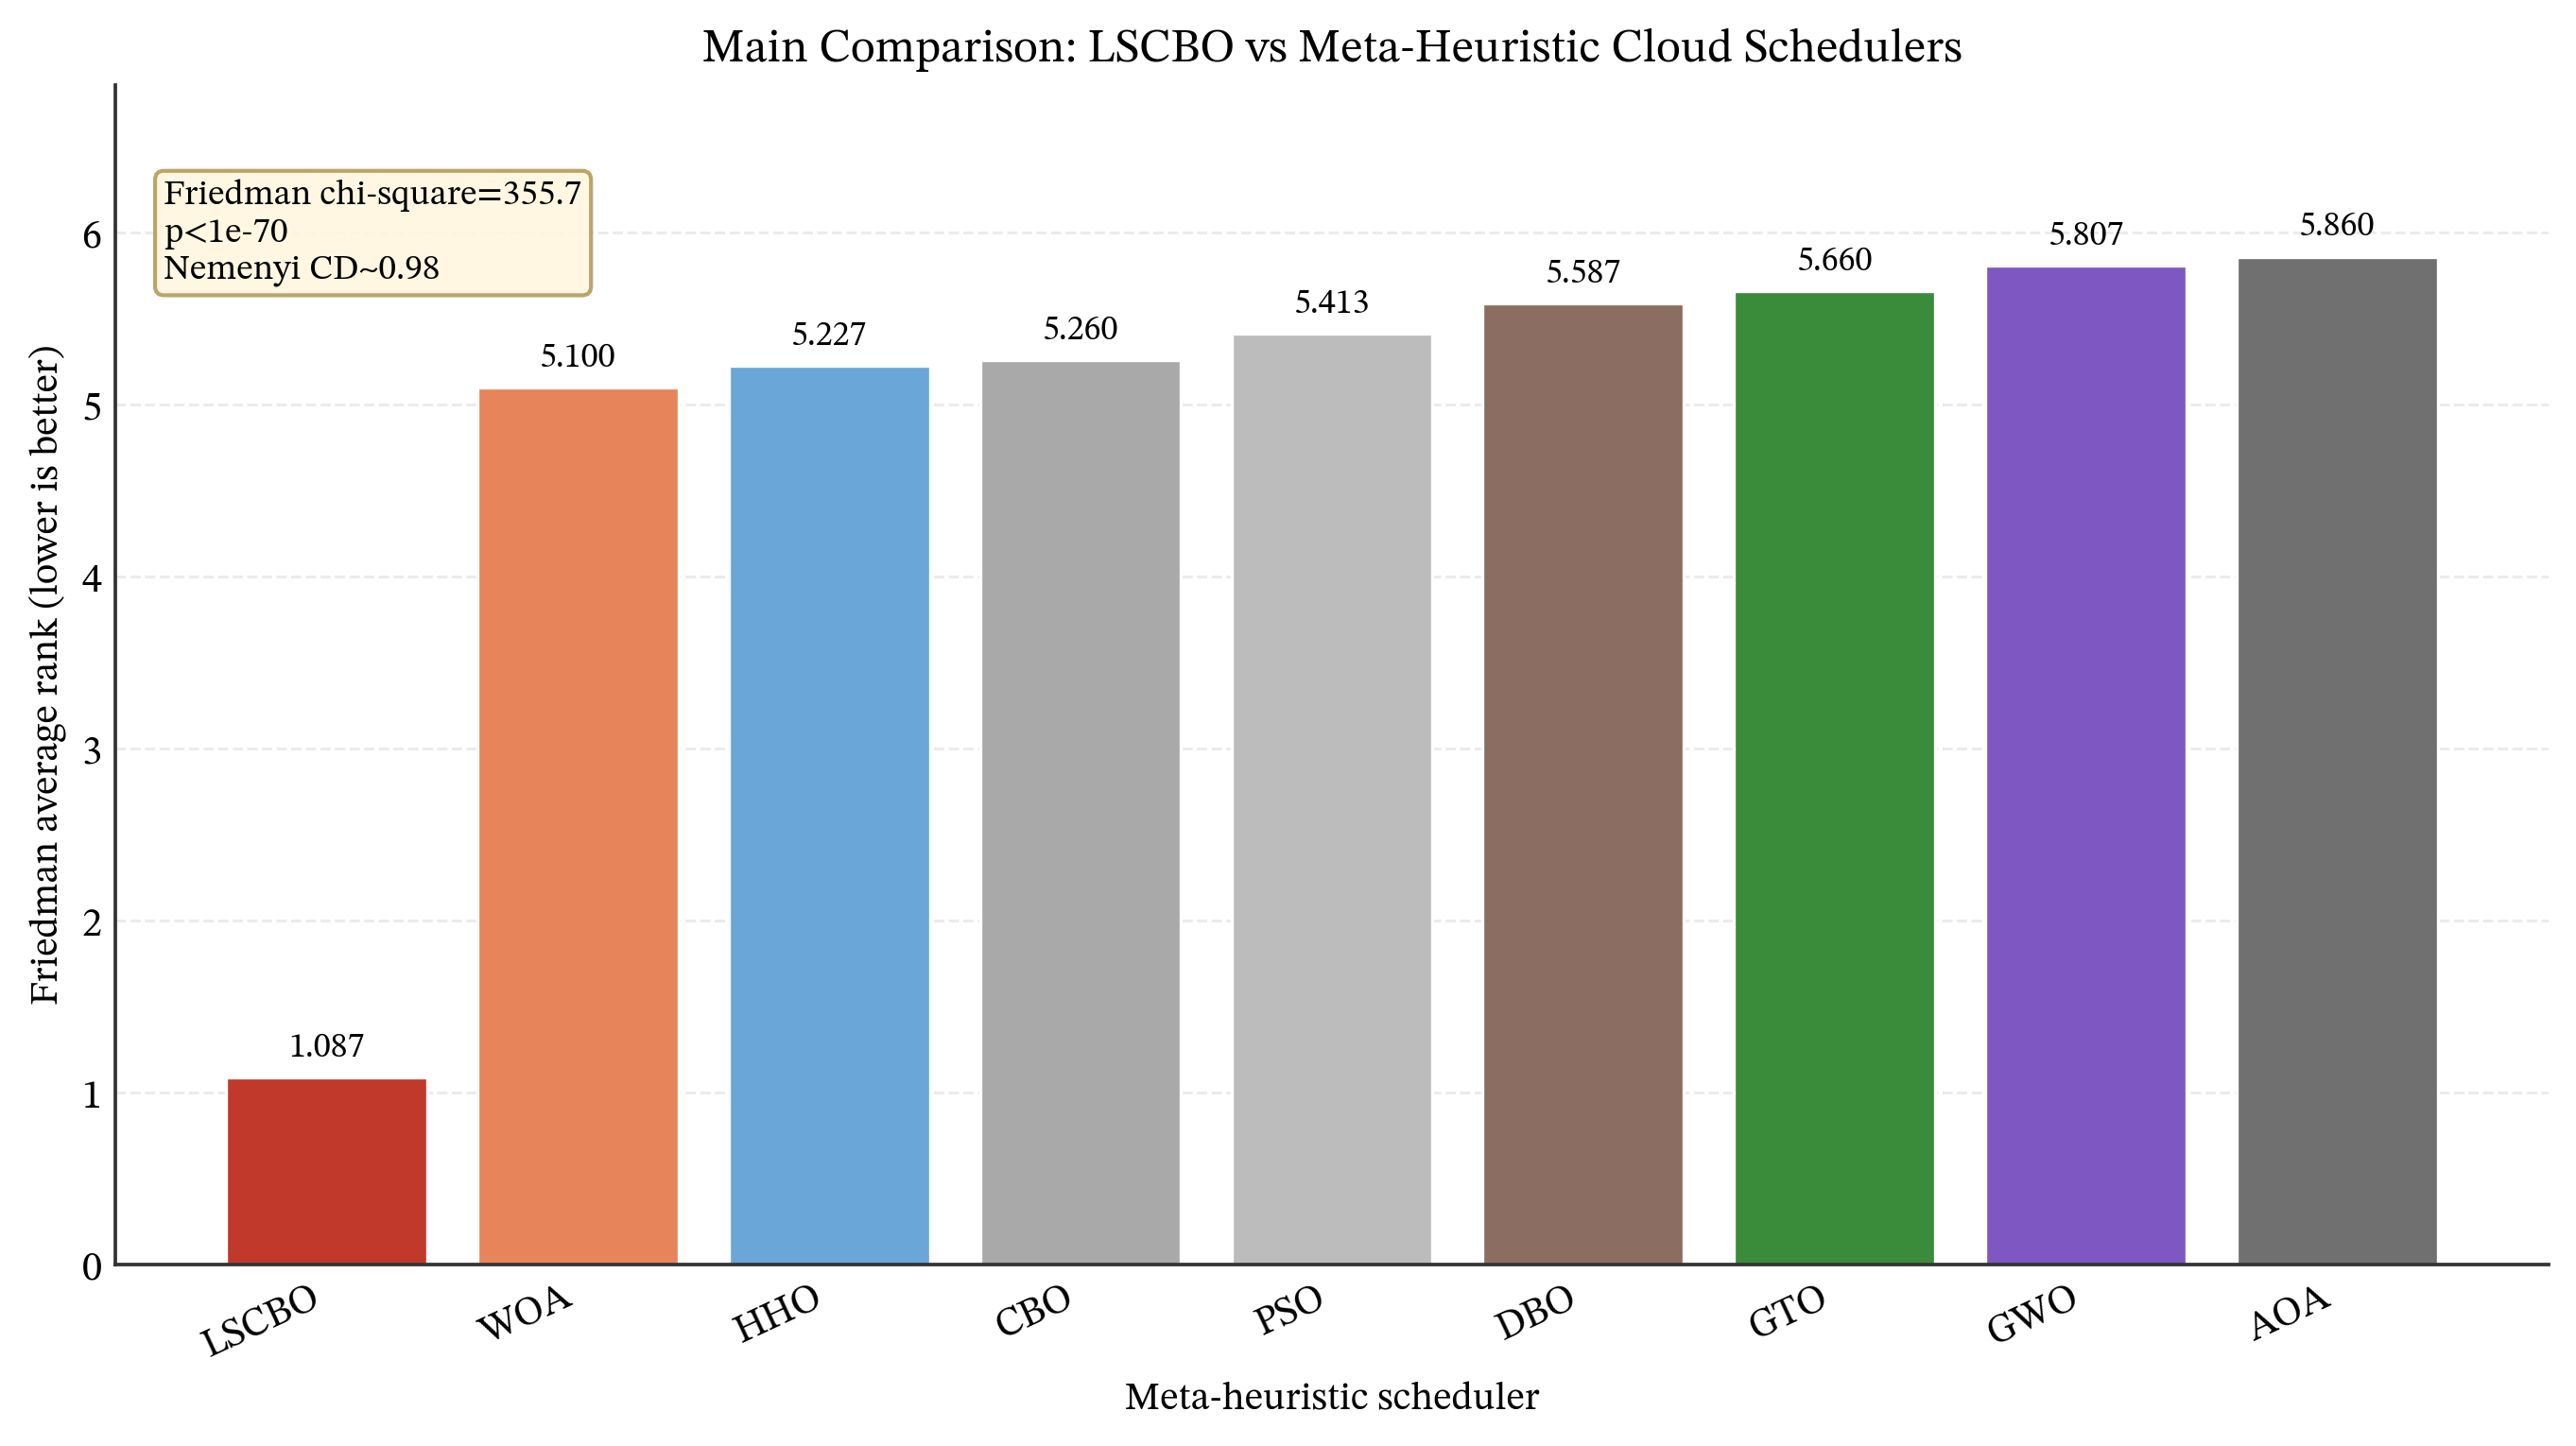
\includegraphics[width=0.85\textwidth]{figures/fig_E4_final_ranking.png}
\caption{Friedman average objective rank across 9 compared meta-heuristic schedulers (150 blocks: 5 scales $\times$ 30 paired seeds). LSCBO obtains the lowest average rank (1.087) within this comparison set (Friedman $\chi^2 = 355.7$, $p < 10^{-70}$, Nemenyi CD $\approx$ 0.98 at $\alpha=0.05$).}\label{fig:friedman_ranking}
\end{figure}

The global Friedman test~\cite{Friedman1937} is applied over $n=150$ blocks (5 task scales $\times$ 30 paired seeds), confirming significant differences among algorithms ($\chi^2 = 355.7$, $p < 10^{-70}$); the resulting average objective ranks are shown in Fig.~\ref{fig:friedman_ranking}. The Iman-Davenport correction~\cite{ImanDavenport1980} yields $F_F \approx 62.8 > F_{0.05}(8, 1192) \approx 1.95$. LSCBO's average objective rank of 1.087 is the lowest within the compared population-based meta-heuristic scheduler family. Table~\ref{tab:wilcoxon} presents pairwise Wilcoxon signed-rank tests~\cite{Wilcoxon1945} with Holm-Bonferroni correction.

\begin{table}[ht]
\centering
\caption{Pairwise Wilcoxon Test on Scalarized Objective (LSCBO vs.\ Each Opponent)}\label{tab:wilcoxon}
\begin{tabular}{l c c c c}
\toprule
\textbf{Opponent} & \textbf{Objective Impr.} & \textbf{$p$ (raw)} & \textbf{$p$ (Holm)} & \textbf{Wins} \\
\midrule
WOA & 15.5\% & $2.54\times10^{-26}$ & $1.95\times10^{-25}$ & 149/150 \\
HHO & 15.5\% & $3.58\times10^{-26}$ & $1.95\times10^{-25}$ & 149/150 \\
CBO (baseline) & 15.6\% & $2.44\times10^{-26}$ & $1.95\times10^{-25}$ & 148/150 \\
PSO & 15.7\% & $2.54\times10^{-26}$ & $1.95\times10^{-25}$ & 148/150 \\
DBO & 15.8\% & $2.59\times10^{-26}$ & $1.95\times10^{-25}$ & 149/150 \\
GTO & 15.8\% & $2.65\times10^{-26}$ & $1.95\times10^{-25}$ & 148/150 \\
GWO & 16.0\% & $2.44\times10^{-26}$ & $1.95\times10^{-25}$ & 148/150 \\
AOA & 16.0\% & $2.44\times10^{-26}$ & $1.95\times10^{-25}$ & 148/150 \\
\bottomrule
\end{tabular}
\smallskip

\footnotesize{Two-sided Wilcoxon signed-rank test over the 150 matched scale--seed blocks; raw $p$-values are Holm-Bonferroni corrected across the eight comparisons. ``Wins'' counts the blocks in which LSCBO attains the lower scalarized objective.}
\end{table}

All pairwise comparisons are statistically significant after Holm-Bonferroni correction (all $p_{\mathrm{Holm}} < 10^{-24}$). The paired win counts show that LSCBO improves the scalarized objective in at least 148 of the 150 matched scale--seed blocks against every opponent. Figure~\ref{fig:makespan_scale} shows the corresponding cross-scale makespan trends for all nine schedulers.

\begin{figure}[htbp]
\centering

\includegraphics[width=0.85\textwidth]{figures/fig_E4_makespan_scale.png}
\caption{Cross-scale makespan trends for all 9 compared meta-heuristic schedulers in the formal 30-seed data. LSCBO maintains the lowest mean makespan across the tested range $N=200$--$5000$.}\label{fig:makespan_scale}
\end{figure}

\subsubsection{Weight Sensitivity Analysis}\label{sec:weight_sensitivity}
To empirically test ranking robustness under alternative scalarization preferences, we conducted a comprehensive weight sensitivity experiment across five configurations (Table~\ref{tab:weight_configs}). The experiment includes the population-based meta-heuristic schedulers across 5 task scales ($N=100$, 300, 500, 800, 1000) with 30 independent runs each.

\begin{table}[ht]
\centering
\caption{Weight Configurations for Sensitivity Analysis}\label{tab:weight_configs}
\begin{tabular}{l c c c c c}
\toprule
\textbf{Config} & $\boldsymbol{w_{ms}}$ & $\boldsymbol{w_{en}}$ & $\boldsymbol{w_{cost}}$ & $\boldsymbol{w_{lb}}$ & \textbf{Description} \\
\midrule
W0 & 0.25 & 0.25 & 0.25 & 0.25 & Equal-weight (baseline) \\
W1 & 0.60 & 0.10 & 0.10 & 0.20 & Makespan-dominant \\
W2 & 0.10 & 0.40 & 0.40 & 0.10 & Energy-cost-balanced \\
W3 & 0.85 & 0.05 & 0.05 & 0.05 & Pure makespan \\
W4 & 0.05 & 0.05 & 0.05 & 0.85 & Pure load-balance \\
\bottomrule
\end{tabular}
\end{table}

\begin{figure}[htbp]
\centering

\includegraphics[width=0.85\textwidth]{figures/fig_E1_rank_heatmap.png}
\caption{Objective-rank heatmap across 5 weight configurations in the formal 30-seed sensitivity data. LSCBO obtains rank 1 under every tested scalarization profile.}\label{fig:weight_heatmap}
\end{figure}

\textbf{Key findings.} LSCBO obtains the best mean scalarized objective under all five weight configurations. This confirms that the primary ranking result is not an artifact of the equal-weight choice. The formal data show the same qualitative ordering when makespan, energy, cost, or load balance is emphasized, with the strongest gains appearing when scheduling pressure is tied to completion time, energy, or load balance. The source values used to generate Fig.~\ref{fig:weight_heatmap} are stored with the formal full-run CSV files to keep the figure reproducible.

\subsubsection{Perturbation Mechanism Comparison}\label{sec:perturbation}
We compared four perturbation mechanisms within the LSCBO framework: (1) L\'{e}vy flight ($\beta=1.5$), (2) Gaussian perturbation, (3) Cauchy perturbation, and (4) random restart ($p=0.05$), together with a no-perturbation baseline. All configurations use the same task scales and seed set (450 trials: 30 seeds $\times$ 3 task scales $\times$ 5 variants).

\begin{table}[ht]
\centering
\caption{Perturbation Mechanism Comparison within the LSCBO Framework}\label{tab:perturbation}
\begin{tabular}{l c c c}
\toprule
\textbf{Variant} & \textbf{Makespan} & \textbf{Objective} & \textbf{Objective order} \\
\midrule
Random restart & 333.3 & 1.390 & 1 \\
None & 331.5 & 1.392 & 2 \\
L\'{e}vy & 333.9 & 1.394 & 3 \\
Cauchy & 335.1 & 1.399 & 4 \\
Gaussian & 333.5 & 1.402 & 5 \\
\bottomrule
\end{tabular}
\end{table}

The perturbation comparison does not support a strong claim that L\'{e}vy flight is independently superior to other perturbation choices. Random restart and even the no-perturbation baseline are numerically close to the L\'{e}vy setting in this diagnostic experiment. Therefore, L\'{e}vy flight is retained in LSCBO as an auxiliary exploration mechanism, while the paper's main empirical claim is assigned to task-reassignment local search.

\subsubsection{Phase~2--3 Isolation Ablation}\label{sec:phase_ablation}
We conducted a targeted ablation experiment using 1050 recorded runs (7 variants $\times$ 5 task scales $\times$ 30 seeds). The table below reports the paired means over 150 matched scale--seed blocks per variant, using the complete LSCBO variant as the reference.

\begin{table}[ht]
\centering
\caption{Formal Component-Ablation Results (vs.\ Complete LSCBO Variant)}\label{tab:phase_ablation}
\begin{tabular}{l c c c c}
\toprule
\textbf{Variant} & \textbf{Makespan} & \textbf{Objective} & $\boldsymbol{\Delta}$ \textbf{Objective} & \textbf{Interpretation} \\
\midrule
LSCBO (complete) & 534.8 & 1.415 & --- & final design \\
LS-only & 545.3 & 1.419 & +0.3\% & local search retained \\
No L\'{e}vy & 534.0 & 1.402 & $-0.9\%$ & perturbation not decisive \\
No local search & 613.4 & 1.642 & +16.0\% & local search removed \\
CBO base & 615.2 & 1.653 & +16.9\% & no LSCBO additions \\
No Phase~2 & 532.1 & 1.392 & $-1.6\%$ & interaction effect \\
No Phase~3 & 536.6 & 1.397 & $-1.3\%$ & interaction effect \\
\bottomrule
\end{tabular}
\end{table}

These ablation results show the clearest degradation when task-reassignment local search is removed: the objective increases by 16.0\% relative to the complete LSCBO variant, and the CBO base variant is similarly worse. By contrast, the no-L\'{e}vy, no-Phase~2, and no-Phase~3 diagnostics are numerically close to, or slightly better than, the complete variant. This result reinforces two points: task reassignment is the robust scheduling-specific contributor, and the remaining CBO-phase and perturbation components interact in a non-additive way rather than producing monotonic gains when each is included.

\subsubsection{VM Heterogeneity Robustness}\label{sec:vm_heterogeneity}
We evaluated the meta-heuristic schedulers across 3 VM configurations (MIPS ratios: 1.5:1, 5:1, and 20:1) at 3 task scales. This experiment is used as a robustness check for the meta-heuristic comparison, not as a claim of dominance over deterministic or learning-based scheduling paradigms.

\begin{table}[ht]
\centering
\caption{Mean Objective Across VM Heterogeneity Configurations}\label{tab:vm_heterogeneity}
\begin{tabular}{l c c c}
\toprule
\textbf{Algorithm} & \textbf{1.5:1} & \textbf{5:1} & \textbf{20:1} \\
\midrule
\textbf{LSCBO} & \textbf{1.065} & \textbf{1.530} & \textbf{2.673} \\
HHO & 1.159 & 1.844 & 3.908 \\
WOA & 1.160 & 1.841 & 3.929 \\
CBO & 1.159 & 1.846 & 3.931 \\
PSO & 1.159 & 1.846 & 3.941 \\
GWO & 1.162 & 1.853 & 3.950 \\
DBO & 1.162 & 1.849 & 3.953 \\
AOA & 1.161 & 1.847 & 3.960 \\
GTO & 1.159 & 1.848 & 3.964 \\
\bottomrule
\end{tabular}
\smallskip
\footnotesize{Lower values indicate better objective. All nine compared meta-heuristic schedulers are shown; each entry is the mean over the heterogeneity protocol (3 task scales $\times$ 30 seeds $=$ 90 runs per cell).}
\end{table}

LSCBO obtains the lowest mean objective under all three VM heterogeneity settings. Its relative advantage is smallest under the near-homogeneous 1.5:1 setting and largest under the 20:1 setting, which is consistent with a scheduling operator that explicitly targets imbalance among heterogeneous VMs.

\section{Discussion}\label{sec6}

\subsection{Performance Analysis}
LSCBO demonstrates a consistent and context-dependent performance profile across the two experimental series. On CEC2017 benchmarks, LSCBO obtains the lowest average rank of 1.86 within the seven-algorithm comparison, with statistically significant wins over CBO, PSO, SA, and GWO ($p < 0.001$) and statistical parity with DE ($p = 0.059$) and GTO ($p = 0.481$), providing a continuous optimization foundation for the scheduling-domain evaluation. In the scheduling domain, LSCBO obtains an average objective rank of 1.087 within the compared population-based meta-heuristic scheduler family, driven primarily by task-reassignment local search---an exploitation mechanism that is specific to task-to-VM assignment.

The multi-cost profile in Fig.~\ref{fig:multicost_profile} clarifies why the local-search mechanism is meaningful for cloud scheduling. Reassigning tasks from heavily loaded VMs can lower the completion-time bottleneck, reduce load imbalance, and indirectly affect the energy and price terms induced by VM utilization. The asymmetric contribution of LSCBO's two enhancements is therefore instructive. In the internal evolution-path diagnostic experiment, inserting task-reassignment local search produces the largest within-path improvement (V2$\rightarrow$V3, +15.4\% in objective), and the component-ablation experiment shows that removing local search increases the objective by 16.0\% relative to the complete LSCBO variant. L\'{e}vy flight provides only a small and unstable contribution in the final scheduling framework. Thus, LSCBO's cloud-scheduling advantage is best interpreted as the combined effect of a CBO search framework and a strong scheduling-specific reassignment operator, with stochastic perturbation serving as an auxiliary component.

The ablation results also caution against treating every added component as independently beneficial. Some reduced variants remain numerically close to the complete LSCBO setting, indicating that CBO phases, stochastic perturbation, and local search interact rather than contributing additively. This is why the paper assigns the core contribution to task-reassignment local search and treats L\'{e}vy perturbation as a secondary search-diversity mechanism.

\subsection{Robustness and Generalizability}
LSCBO's performance advantage within the meta-heuristic scheduler comparison is robust across a wide range of experimental conditions. The weight sensitivity analysis confirms that LSCBO obtains the best objective rank under all five scalarization configurations. The VM heterogeneity analysis demonstrates that LSCBO has the lowest mean objective across MIPS ratios from 1.5:1 to 20:1. These findings suggest that LSCBO's contribution is not an artifact of a single weight setting or VM configuration, while leaving broader cross-paradigm comparisons as a separate empirical question.

\subsection{Limitations}
Several limitations should be considered. First, the reported multi-cost metrics are computed from an analytic task/VM model; although all 12,780 formal rows were executed and confirmed to complete under a full CloudSim Plus simulation, the simulator uses a TimeShared scheduling policy and a linear power model, so the absolute cost values remain model-dependent and could shift under alternative simulator configurations or real datacenter telemetry. Second, the current power model is linear, which induces a structural dependence between makespan and energy; nonlinear power models would be needed to fully decouple these objectives. Relatedly, because all schedulers execute the same task set on the same VM-price model, the execution-cost component varies only marginally across methods (Table~\ref{tab:per_scale_cbo}) and contributes little discriminative signal to the scalarized objective; the observed advantage is therefore driven primarily by makespan, energy, and load balance rather than by cost. Third, following the standard format of cloud meta-heuristic scheduling studies, the main comparison focuses on population-based meta-heuristic schedulers rather than exact optimization, dispatching rules, or DRL-based schedulers; these provide useful boundary baselines but are outside the main comparative scope of this paper. Therefore, the results should be read as evidence of better performance within the evaluated cloud meta-heuristic scheduler family, not as a universal state-of-the-art claim across all scheduling paradigms. Fourth, the offline batch scheduling assumption limits direct applicability to dynamic online cloud environments because the present task-reassignment operator performs pre-execution assignment rather than runtime task migration. Fifth, the task-reassignment local search has been validated primarily within the CBO framework; its transferability to other meta-heuristics (GTO, PSO, GWO) remains an open empirical question.

\section{Conclusion}\label{sec7}

This paper proposed LSCBO, a CBO-based scheduler that combines task-reassignment local search with L\'{e}vy-assisted stochastic exploration for multi-cost cloud task scheduling. The algorithm was comprehensively evaluated through two experimental series: (1) 29 CEC2017 global optimization functions to validate its fundamental optimization capability, and (2) formal multi-cost scheduling experiments across 5 task scales, 5 weight configurations, 3 VM heterogeneity regimes, component-level ablation, and perturbation mechanism comparisons.

The experimental results demonstrate that:
\begin{itemize}
    \item LSCBO obtains the lowest average objective rank of 1.087 among the nine compared population-based meta-heuristic schedulers ($p < 10^{-70}$), with per-scale objective improvements of 7.4\%--22.6\% and makespan improvements of 9.6\%--30.1\% over the standardized CBO baseline.
    \item On CEC2017 benchmarks, LSCBO obtains the lowest Friedman average rank of 1.86 among seven compared algorithms, with statistically significant wins over CBO, PSO, SA, and GWO ($p < 0.001$) and statistical parity with DE ($p = 0.059$) and GTO ($p = 0.481$).
    \item The task-reassignment local search is the dominant performance driver, while stochastic perturbation provides a smaller and less stable auxiliary benefit.
    \item LSCBO's ranking advantage within the evaluated meta-heuristic scheduler family is robust across all tested weight configurations and VM heterogeneity regimes.
    \item The evolution-path methodology provides an evidence-based approach for component-level ablation in meta-heuristic research.
\end{itemize}

Future work should: (1) implement Pareto-front methods to explore multi-objective trade-offs beyond single-point scalarization, (2) test the transferability of task-reassignment local search to other meta-heuristics, (3) investigate nonlinear power models to decouple makespan and energy objectives, (4) extend cost-decomposition curves across additional task scales and dynamic workload settings, (5) add a separate boundary-baseline study against dispatching rules, DRL-based schedulers, and exact or near-exact small-instance solvers, and (6) evaluate on real-world cloud workload traces with diverse distributional characteristics.

\section*{Statements and Declarations}
\textbf{Funding} No external funding was received for this work.

\textbf{Competing Interests} The authors declare no competing interests.

\textbf{Data Availability} The CSV files used to generate the current manuscript tables and figures, including the formal 12,780-row multi-cost comparison (with every row validated through a full CloudSim Plus simulation), evolution-path analysis, component-ablation analysis, CEC2017 ranking, weight-sensitivity data, VM heterogeneity data, and perturbation diagnostics, are organized with recomputation scripts and are deposited in the public project repository (\url{https://github.com/Lazywords2006/LSCBO}); they are additionally available from the corresponding author upon reasonable request during review.

\textbf{Code Availability} The LSCBO optimizer implementation, CloudSim Plus experiment entry points, result-aggregation scripts, and figure-generation scripts used in this study are publicly available at \url{https://github.com/Lazywords2006/LSCBO} to support reproducibility.

\textbf{Ethics Approval} Not applicable.

\textbf{Consent to Participate} Not applicable.

\textbf{Consent for Publication} Not applicable.

\begin{thebibliography}{64}

\bibitem{Braun2001}
Braun TD, Siegel HJ, Beck N, B\"{o}l\"{o}ni LL, Maheswaran M, Reuther AI, Robertson JP, Theys MD, Yao B, Hensgen D, Freund RF. A comparison of eleven static heuristics for mapping a class of independent tasks onto heterogeneous distributed computing systems. \textit{J Parallel Distrib Comput}, 61(6):810--837 (2001). \url{https://doi.org/10.1006/jpdc.2000.1714}

\bibitem{Kiliaan1991}
Kiliaan H, Mamo C, Paquet P. A coyote, \textit{Canis latrans}, and badger, \textit{Taxidea taxus}, interaction near Cypress Hills Provincial Park, Alberta. \textit{Can Field-Nat}, 105(1):122--123 (1991). \url{https://doi.org/10.5962/p.357965}

\bibitem{Etminani2007}
Etminani K, Naghibzadeh M. A Min-Min Max-Min selective algorithm for grid task scheduling. \textit{Proc 3rd IEEE/IFIP Int Conf Cent Asia Internet}, 1--7 (2007). \url{https://doi.org/10.1109/CANET.2007.4401694}

\bibitem{Kennedy1995}
Kennedy J, Eberhart R. Particle swarm optimization. \textit{Proc ICNN'95-Int Conf Neural Networks}, 4:1942--1948 (1995). \url{https://doi.org/10.1109/ICNN.1995.488968}

\bibitem{Goldberg1989}
Goldberg DE. Genetic algorithms in search, optimization, and machine learning. \textit{Addison-Wesley} (1989).

\bibitem{Storn1997}
Storn R, Price K. Differential evolution---a simple and efficient heuristic for global optimization over continuous spaces. \textit{J Glob Optim}, 11(4):341--359 (1997). \url{https://doi.org/10.1023/A:1008202821328}

\bibitem{Tasgetiren2007}
Tasgetiren MF, Liang YC, \c{S}evkli M, Gencyilmaz G. A particle swarm optimization algorithm for makespan and total flowtime minimization in the permutation flowshop sequencing problem. \textit{Eur J Oper Res}, 177(3):1930--1947 (2007). \url{https://doi.org/10.1016/j.ejor.2005.12.024}

\bibitem{Mantegna1994}
Mantegna RN. Fast, accurate algorithm for numerical simulation of L\'{e}vy stable stochastic processes. \textit{Phys Rev E}, 49(5):4677--4683 (1994). \url{https://doi.org/10.1103/PhysRevE.49.4677}

\bibitem{Yang2009}
Yang XS, Deb S. Cuckoo search via L\'{e}vy flights. \textit{Proc 2009 World Congr Nat Biol Inspired Comput (NaBIC)}, 210--214 (2009). \url{https://doi.org/10.1109/NABIC.2009.5393690}

\bibitem{Heidari2019}
Heidari AA, Mirjalili S, Faris H, Aljarah I, Mafarja M, Chen H. Harris hawks optimization: algorithm and applications. \textit{Future Gener Comput Syst}, 97:849--872 (2019). \url{https://doi.org/10.1016/j.future.2019.02.028}

\bibitem{Mirjalili2016}
Mirjalili S, Lewis A. The whale optimization algorithm. \textit{Adv Eng Softw}, 95:51--67 (2016). \url{https://doi.org/10.1016/j.advengsoft.2016.01.008}

\bibitem{Xue2022}
Xue J, Shen B. Dung beetle optimizer: a new meta-heuristic algorithm for global optimization. \textit{J Supercomput}, 79:7305--7336 (2023). \url{https://doi.org/10.1007/s11227-022-04959-6}

\bibitem{Deng2023}
Deng L, Liu S. Snow ablation optimizer: a novel metaheuristic technique for numerical optimization and engineering design. \textit{Expert Syst Appl}, 225:120069 (2023). \url{https://doi.org/10.1016/j.eswa.2023.120069}

\bibitem{AbdelBasset2023}
Abdel-Basset M, Mohamed R, Azeem SAA, Jameel M, Abouhawwash M. Kepler optimization algorithm: a new metaheuristic algorithm inspired by Kepler's laws of planetary motion. \textit{Knowl-Based Syst}, 268:110454 (2023). \url{https://doi.org/10.1016/j.knosys.2023.110454}

\bibitem{Qian2025}
Qian Z, Zhang Y, Pu D, Xie G, Pu D, Ye M. A new hybrid improved Kepler optimization algorithm based on multi-strategy fusion and its applications. \textit{Mathematics}, 13(3):405 (2025). \url{https://doi.org/10.3390/math13030405}

\bibitem{Abualigah2021}
Abualigah L, Diabat A, Mirjalili S, Elaziz MA, Gandomi AH. The arithmetic optimization algorithm. \textit{Comput Methods Appl Mech Eng}, 376:113609 (2021). \url{https://doi.org/10.1016/j.cma.2020.113609}

\bibitem{Hashim2022}
Hashim FA, Hussien AG. Snake optimizer: a novel meta-heuristic optimization algorithm. \textit{Knowl-Based Syst}, 242:108320 (2022). \url{https://doi.org/10.1016/j.knosys.2022.108320}

\bibitem{Trojovska2022}
Trojovsk\'{y} P, Dehghani M. Pelican optimization algorithm: a novel nature-inspired algorithm for engineering applications. \textit{Sensors}, 22(3):855 (2022). \url{https://doi.org/10.3390/s22030855}

\bibitem{Faramarzi2020}
Faramarzi A, Heidarinejad M, Mirjalili S, Gandomi AH. Marine Predators Algorithm: a nature-inspired metaheuristic. \textit{Expert Syst Appl}, 152:113377 (2020). \url{https://doi.org/10.1016/j.eswa.2020.113377}

\bibitem{Abualigah2022}
Abualigah L, Elaziz MA, Sumari P, Geem ZW, Gandomi AH. Reptile Search Algorithm (RSA): a nature-inspired meta-heuristic optimizer. \textit{Expert Syst Appl}, 191:116158 (2022). \url{https://doi.org/10.1016/j.eswa.2021.116158}

\bibitem{Wang2022}
Wang L, Cao Q, Zhang Z, Mirjalili S, Zhao W. Artificial rabbits optimization: a new bio-inspired meta-heuristic algorithm for solving engineering optimization problems. \textit{Eng Appl Artif Intell}, 114:105082 (2022). \url{https://doi.org/10.1016/j.engappai.2022.105082}

\bibitem{Dehghani2023}
Dehghani M, Trojovsk\'{y} P. Osprey optimization algorithm: a new bio-inspired metaheuristic algorithm for solving engineering optimization problems. \textit{Front Mech Eng}, 8:1126450 (2023). \url{https://doi.org/10.3389/fmech.2022.1126450}

\bibitem{Chintale2024}
Chintale P, Malviya RK, Merla NB, Chinna PPG, Desaboyina G, Sure TAR. Levy flight osprey optimization algorithm for task scheduling in cloud computing. \textit{Proc 2024 Int Conf Intell Algorithms Comput Intell Syst (IACIS)}, 1--5 (2024). \url{https://doi.org/10.1109/IACIS61494.2024.10721633}

\bibitem{Khatab2025}
Khatab M, El-Gamel M, Saleh AI, El-Shenawy A, Rabie AH. Coyote and Badger Optimization (CBO): a natural inspired meta-heuristic algorithm based on cooperative hunting. \textit{Commun Nonlinear Sci Numer Simul}, 140:108333 (2025). \url{https://doi.org/10.1016/j.cnsns.2024.108333}

\bibitem{Xie2024}
Xie R, Li S, Wu F, Wu L, Xiong X. An enhanced dung beetle optimizer for cloud task schedule. \textit{Proc 4th Int Conf Appl Math Model Intell Comput (CAMMIC 2024)}, 13219:80 (2024). \url{https://doi.org/10.1117/12.3036506}

\bibitem{Ghafari2023}
Ghafari R, Mansouri N. E-AVOA-TS: enhanced African vultures optimization algorithm-based task scheduling strategy for fog--cloud computing. \textit{Sustain Comput Inform Syst}, 40:100918 (2023). \url{https://doi.org/10.1016/j.suscom.2023.100918}

\bibitem{Rengaraj2023}
Rengaraj alias Muralidharan R, Latha K. Gorilla troops optimizer based fault tolerant aware scheduling scheme for cloud environment. \textit{Intell Autom Soft Comput}, 35(2):1923--1937 (2023). \url{https://doi.org/10.32604/iasc.2023.029495}

\bibitem{Ferahtia2023}
Ferahtia S, Houari A, Rezk H, Djerioui A, Machmoum M, Motahhir S, Ait-Ahmed M. Red-tailed hawk algorithm for numerical optimization and real-world problems. \textit{Sci Rep}, 13:12950 (2023). \url{https://doi.org/10.1038/s41598-023-38778-3}

\bibitem{Qin2024}
Qin X, Li S, Tong J, Xie C, Zhang X, Wu F, Xie Q, Ling Y, Lin G. ERTH scheduler: enhanced red-tailed hawk algorithm for multi-cost optimization in cloud task scheduling. \textit{Artif Intell Rev}, 57:328 (2024). \url{https://doi.org/10.1007/s10462-024-10945-6}

\bibitem{EbrahimiMood2025}
Ebrahimi Mood S, Souri A, Inanc N, Li KC. CEEO: an innovative Coulomb-enhanced equilibrium optimizer for task scheduling of cloud services in IoT environments. \textit{Computing}, 107:138 (2025). \url{https://doi.org/10.1007/s00607-025-01495-y}

\bibitem{Gunduz2025}
Gunduz A, Senan S, Gurkas-Aydin Z. A hybrid DECSO algorithm for efficient multi-objective task scheduling in cloud computing environments. \textit{Cluster Comput}, 28:848 (2025). \url{https://doi.org/10.1007/s10586-025-05586-5}

\bibitem{Sabipour2025}
Sabipour MR, Sayadnavard MH. A chaotic RIME optimization algorithm based on generalized quadratic interpolation with L\'{e}vy flight for task scheduling in cloud computing. \textit{J Soft Comput Inf Technol}, 14(1):57--67 (2025). \url{https://doi.org/10.22034/jscit.2025.220413}

\bibitem{Zhu2025}
Zhu M, Li J, Yang X. A hybrid SAO and RIME optimizer for global optimization and cloud task scheduling. \textit{Biomimetics}, 10(10):690 (2025). \url{https://doi.org/10.3390/biomimetics10100690}

\bibitem{Abdollahzadeh2021}
Abdollahzadeh B, Soleimanian Gharehchopogh F, Mirjalili S. Artificial gorilla troops optimizer: a new nature-inspired metaheuristic algorithm for global optimization problems. \textit{Int J Intell Syst}, 36:5887--5958 (2021). \url{https://doi.org/10.1002/int.22535}

\bibitem{Mirjalili2014}
Mirjalili S, Mirjalili SM, Lewis A. Grey wolf optimizer. \textit{Adv Eng Softw}, 69:46--61 (2014). \url{https://doi.org/10.1016/j.advengsoft.2013.12.007}

\bibitem{Moscato1989}
Moscato P. On evolution, search, optimization, genetic algorithms and martial arts: towards memetic algorithms. \textit{Caltech Concurrent Computation Program, C3P Report 826} (1989).

\bibitem{Mao2019}
Mao H, Schwarzkopf M, Bojja Venkatakrishnan S, Meng Z, Alizadeh M. Learning scheduling algorithms for data processing clusters. \textit{Proc ACM SIGCOMM 2019}, 270--288 (2019). \url{https://doi.org/10.1145/3341302.3342080}

\bibitem{Mao2016}
Mao H, Alizadeh M, Menache I, Kandula S. Resource management with deep reinforcement learning. \textit{Proc 15th ACM Workshop Hot Topics Netw (HotNets)}, 50--56 (2016). \url{https://doi.org/10.1145/3005745.3005750}

\bibitem{Deb2002}
Deb K, Pratap A, Agarwal S, Meyarivan T. A fast and elitist multiobjective genetic algorithm: NSGA-II. \textit{IEEE Trans Evol Comput}, 6(2):182--197 (2002). \url{https://doi.org/10.1109/4235.996017}

\bibitem{Zhang2007}
Zhang Q, Li H. MOEA/D: a multiobjective evolutionary algorithm based on decomposition. \textit{IEEE Trans Evol Comput}, 11(6):712--731 (2007). \url{https://doi.org/10.1109/TEVC.2007.892759}

\bibitem{Calheiros2011}
Calheiros RN, Ranjan R, Beloglazov A, De Rose CAF, Buyya R. CloudSim: a toolkit for modeling and simulation of cloud computing environments and evaluation of resource provisioning algorithms. \textit{Softw Pract Exp}, 41(1):23--50 (2011). \url{https://doi.org/10.1002/spe.995}

\bibitem{SilvaFilho2017}
Silva Filho MC, Oliveira RL, Monteiro CC, Inacio PRM, Freire MM. CloudSim Plus: a cloud computing simulation framework pursuing software engineering principles for improved modularity, extensibility and correctness. \textit{Proc 2017 IFIP/IEEE Symp Integr Netw Serv Manag (IM)}, 400--406 (2017). \url{https://doi.org/10.23919/INM.2017.7987304}

\bibitem{Tanabe2014}
Tanabe R, Fukunaga AS. Improving the search performance of SHADE using linear population size reduction. \textit{Proc 2014 IEEE Congr Evol Comput (CEC)}, 1658--1665 (2014). \url{https://doi.org/10.1109/CEC.2014.6900380}

\bibitem{Hansen2001}
Hansen N, Ostermeier A. Completely derandomized self-adaptation in evolution strategies. \textit{Evol Comput}, 9(2):159--195 (2001). \url{https://doi.org/10.1162/106365601750190398}

\bibitem{Demsar2006}
Dem{\v s}ar J. Statistical comparisons of classifiers over multiple data sets. \textit{J Mach Learn Res}, 7:1--30 (2006).

\bibitem{Friedman1937}
Friedman M. The use of ranks to avoid the assumption of normality implicit in the analysis of variance. \textit{J Am Stat Assoc}, 32(200):675--701 (1937). \url{https://doi.org/10.1080/01621459.1937.10503522}

\bibitem{Wilcoxon1945}
Wilcoxon F. Individual comparisons by ranking methods. \textit{Biometrics Bull}, 1(6):80--83 (1945). \url{https://doi.org/10.2307/3001968}

\bibitem{ImanDavenport1980}
Iman RL, Davenport JM. Approximations of the critical region of the Friedman statistic. \textit{Commun Stat--Theory Methods}, 9(6):571--595 (1980). \url{https://doi.org/10.1080/03610928008827904}


\bibitem{Kirkpatrick1983}
Kirkpatrick S, Gelatt Jr CD, Vecchi MP. Optimization by simulated annealing. \textit{Science}, 220(4598):671--680 (1983). \url{https://doi.org/10.1126/science.220.4598.671}

\bibitem{CEC2017}
Awad NH, Ali MZ, Liang JJ, Qu BY, Suganthan PN. Problem definitions and evaluation criteria for the CEC 2017 special session and competition on single objective bound constrained real-parameter numerical optimization. \textit{Nanyang Technological University}, Tech. Rep. (2016).

\end{thebibliography}

\end{document}
